\chapter{Precoding under Outdated CSI}
\label{chapter:precoding_under_outdated_csi}

% intro
In Chapter~\ref{chapter:mu_mimo_precoding}, linear precoding was developed under the implicit assumption that the \ac{CSI} used to design the precoder coincides with the \ac{CSI} experienced by the \acp{UT} at the moment of transmission.
As discussed in Chapter~\ref{chapter:hts_communication_systems}, this assumption breaks down in the mobile satellite scenario considered in this work, owing to the combination of a large propagation delay and a \ac{UT}-induced Doppler spread.
This chapter is devoted to characterizing the impact of this mismatch on precoder performance and to developing a strategy that compensates for it.

% roadmap
Section~\ref{section:outdated_csi_problem_formulation} formulates the problem precisely and introduces the \ac{CSI} feedback delay as the key operating parameter. From there, the chapter proceeds in three steps.
First, Section~\ref{section:outdated_csi_impact} quantifies the impact of outdated \ac{CSI} on the achievable rate of the linear precoders developed in Chapter~\ref{chapter:mu_mimo_precoding}.
Section~\ref{section:outdated_csi_compensation} then proposes a compensation method that exploits the temporal correlation of the channel in order to predict the instantaneous channel at the time of transmission.
Finally, Section~\ref{section:realistic_channel_evaluation} re-evaluates both the impact of outdated \ac{CSI} and the proposed compensation strategy under a more realistic channel model.

% conclusion
To end this work, the results are applied to a set of representative example scenarios, after which the main findings are summarized in a final conclusion.

\section{Problem Formulation}
\label{section:outdated_csi_problem_formulation}
% ============================
%     Problem Formulation
% ============================

We consider the forward link of the multi-beam \ac{HTS} system as described in Chapter~\ref{chapter:hts_communication_systems}. 
The \ac{GW} serves $K$ \acp{UT} simultaneously through the satellite, equipped with $N_T$ feeds, by applying a linear precoder to the data symbols.
Each \ac{UT} is equipped with $N_R$ receive antennas.
The simulations performed in this chapter focus on a system in which the \ac{BS} has $8$ transmit antennas and serves $4$ \acp{UT} with $2$ receive antennas each.
The channel of \ac{UT}~$k$ at time $t$ is denoted by $\mathbf{H}_k(t) \in \mathbb{C}^{N_R \times N_T}$ and follows the Rician model from~\eqref{eq:rician_channel_model}.
The received signal at \ac{UT}~$k$ reads
\begin{equation}
\label{eq:outdated_csi_received_signal}
    \mathbf{y}_k(t) = \mathbf{H}_k(t)\;\mathbf{F}(t)\,\mathbf{a}(t) + \mathbf{n}_k(t),
\end{equation}
where $\mathbf{a}(t)$ collects the data symbols of each stream intended for \ac{UT}~$k$ into a column vector, and $\mathbf{n}_k(t) \sim \mathcal{CN}(\mathbf{0}, N_0 \mathbf{I}_{N_R})$ is additive noise.
The precoder satisfies the total transmit-power constraint $\mathrm{tr}\big(\mathbf{F}(t)\mathbf{F}^{\mathsf{H}}(t)\big) \leq P_T$ at any moment in time.

In practice, the channel must first be estimated at the \acp{UT} and fed back to the \ac{GW}, before it can be used to design the precoder.
Denoting the aggregate elapsed time by the \ac{CSI} feedback delay~$\tau_{\mathrm{CSI}}$, the precoder applied at time $t$ is necessarily based on the outdated channel state $\mathbf{H}(t - \tau_{\mathrm{CSI}})$.
How severely this mismatch degrades performance depends on how much the channel has evolved during $\tau_{\mathrm{CSI}}$.

The temporal variability of the channel is characterised through the normalised autocorrelation function of its \ac{NLoS} component, denoted by $R_h(\tau)$.
It is shown in Appendix~\ref{appendix_section:doppler_spectrum} that, under Jakes' model, the autocorrelation between two channel realizations separated by a lag $\tau$ equals the zeroth-order Bessel function of the first kind, evaluated in $2\pi f_D \tau$.
The coherence time of the \ac{NLoS} component is defined as the lag at which the autocorrelation first falls to one half of its peak value:
\begin{equation}
\label{eq:coherence_time_def}
    T_c \;\triangleq\; \max\{\tau > 0 \,:\, R_h(\tau) \geq \frac{1}{2}\}.
\end{equation}

Rather than studying the impact of $\tau_{\mathrm{CSI}}$ in absolute terms, the \ac{CSI} feedback delay is expressed as a fraction of the coherence time throughout the analysis.
Two operating points sharing the same $\tau_{\mathrm{CSI}} / T_c$ exhibit, by construction, the same correlation between the outdated and the instantaneous channel, irrespective of the absolute values of $\tau_{\mathrm{CSI}}$ and $T_c$. 
Reporting results as a function of $\tau_{\mathrm{CSI}} / T_c$ therefore yields conclusions that apply to any combination of carrier frequency, \ac{UT} velocity and orbital altitude consistent with the underlying Rician model.

\section{Impact of Outdated CSI}
\label{section:outdated_csi_impact}
% ==============================
%    Impact of Outdated CSI
% ==============================

% intro
In order to quantify the impact of outdated \ac{CSI} on the system performance, the achievable rate obtained by linear precoders developed in Chapter~\ref{chapter:mu_mimo_precoding} is simulated as a function of the \ac{SNR}.
Each precoder is designed based on the outdated channel state $\mathbf{H}(t - \tau_{\mathrm{CSI}})$ and applied to the instantaneous channel $\mathbf{H}(t)$. The resulting sum rate is averaged over more than $100$ channel realizations, and over multiple coherence periods of the fading process for each realization.
Figures~\ref{fig:impact_outdated_csi_achievable_rate_zf_bd} and~\ref{fig:impact_outdated_csi_achievable_rate_wmmse} report the results for a \ac{CSI} feedback delay $\tau_{\mathrm{CSI}}$ that varies from $0 \, T_c$ (instantaneous \ac{CSI}, used as a reference) up to $5/4\, T_c$, slightly beyond the coherence time.

% general observations
All three precoders are very sensitive to outdated \ac{CSI}. Even a delay of only a quarter of the coherence time causes a substantial loss on the achievable rate at moderate and high \ac{SNR} values. 
The loss with respect to instantaneous \ac{CSI} grows monotonically with $\tau_{\mathrm{CSI}}/T_c$, confirming the intuition that the more outdated the \ac{CSI}, the worse the performance.
Once the \ac{CSI} feedback delay surpasses the coherence time of the \ac{NLoS} component, the system becomes essentially unusable.
This aligns with the definition of $T_c$.
Beyond the point $\tau_{\mathrm{CSI}} \geq T_c$, the channel available at the \ac{GW} and the channel actually experienced by the \acp{UT} are only weakly correlated such that the precoder is in effect designed for a channel that bears little resemblance to the true one.
As a consequence, the precoder fails to exploit the spatial dimension of the channel and the sum-rate collapses.

% ZF and BD
A closer look at Figure~\ref{fig:impact_outdated_csi_achievable_rate_zf_bd} shows that both \ac{ZF} and \ac{BD} precoding saturate at high \ac{SNR} once the \ac{CSI} is even slightly outdated.
Both \ac{ZF} and \ac{BD} precoders completely eliminate the interference between the users, no matter the ratio of the transmit power to the noise power.
With outdated \ac{CSI}, the precoder nulls interference along the wrong directions, leaving a residual inter-user interference that is proportional to the transmit power.
As the \ac{SNR} increases, the system transitions from a noise-limited regime to an interference-limited one and the desired signal and the residual interference grow at the same rate.
Therefore, the \ac{SINR} saturates and the achievable rate converges to a finite ceiling, that is determined solely by the magnitude of the channel evolution over the feedback delay.

\begin{figure}[!htb]
    \centering
    \begin{subfigure}{0.495\textwidth}
        \centering
        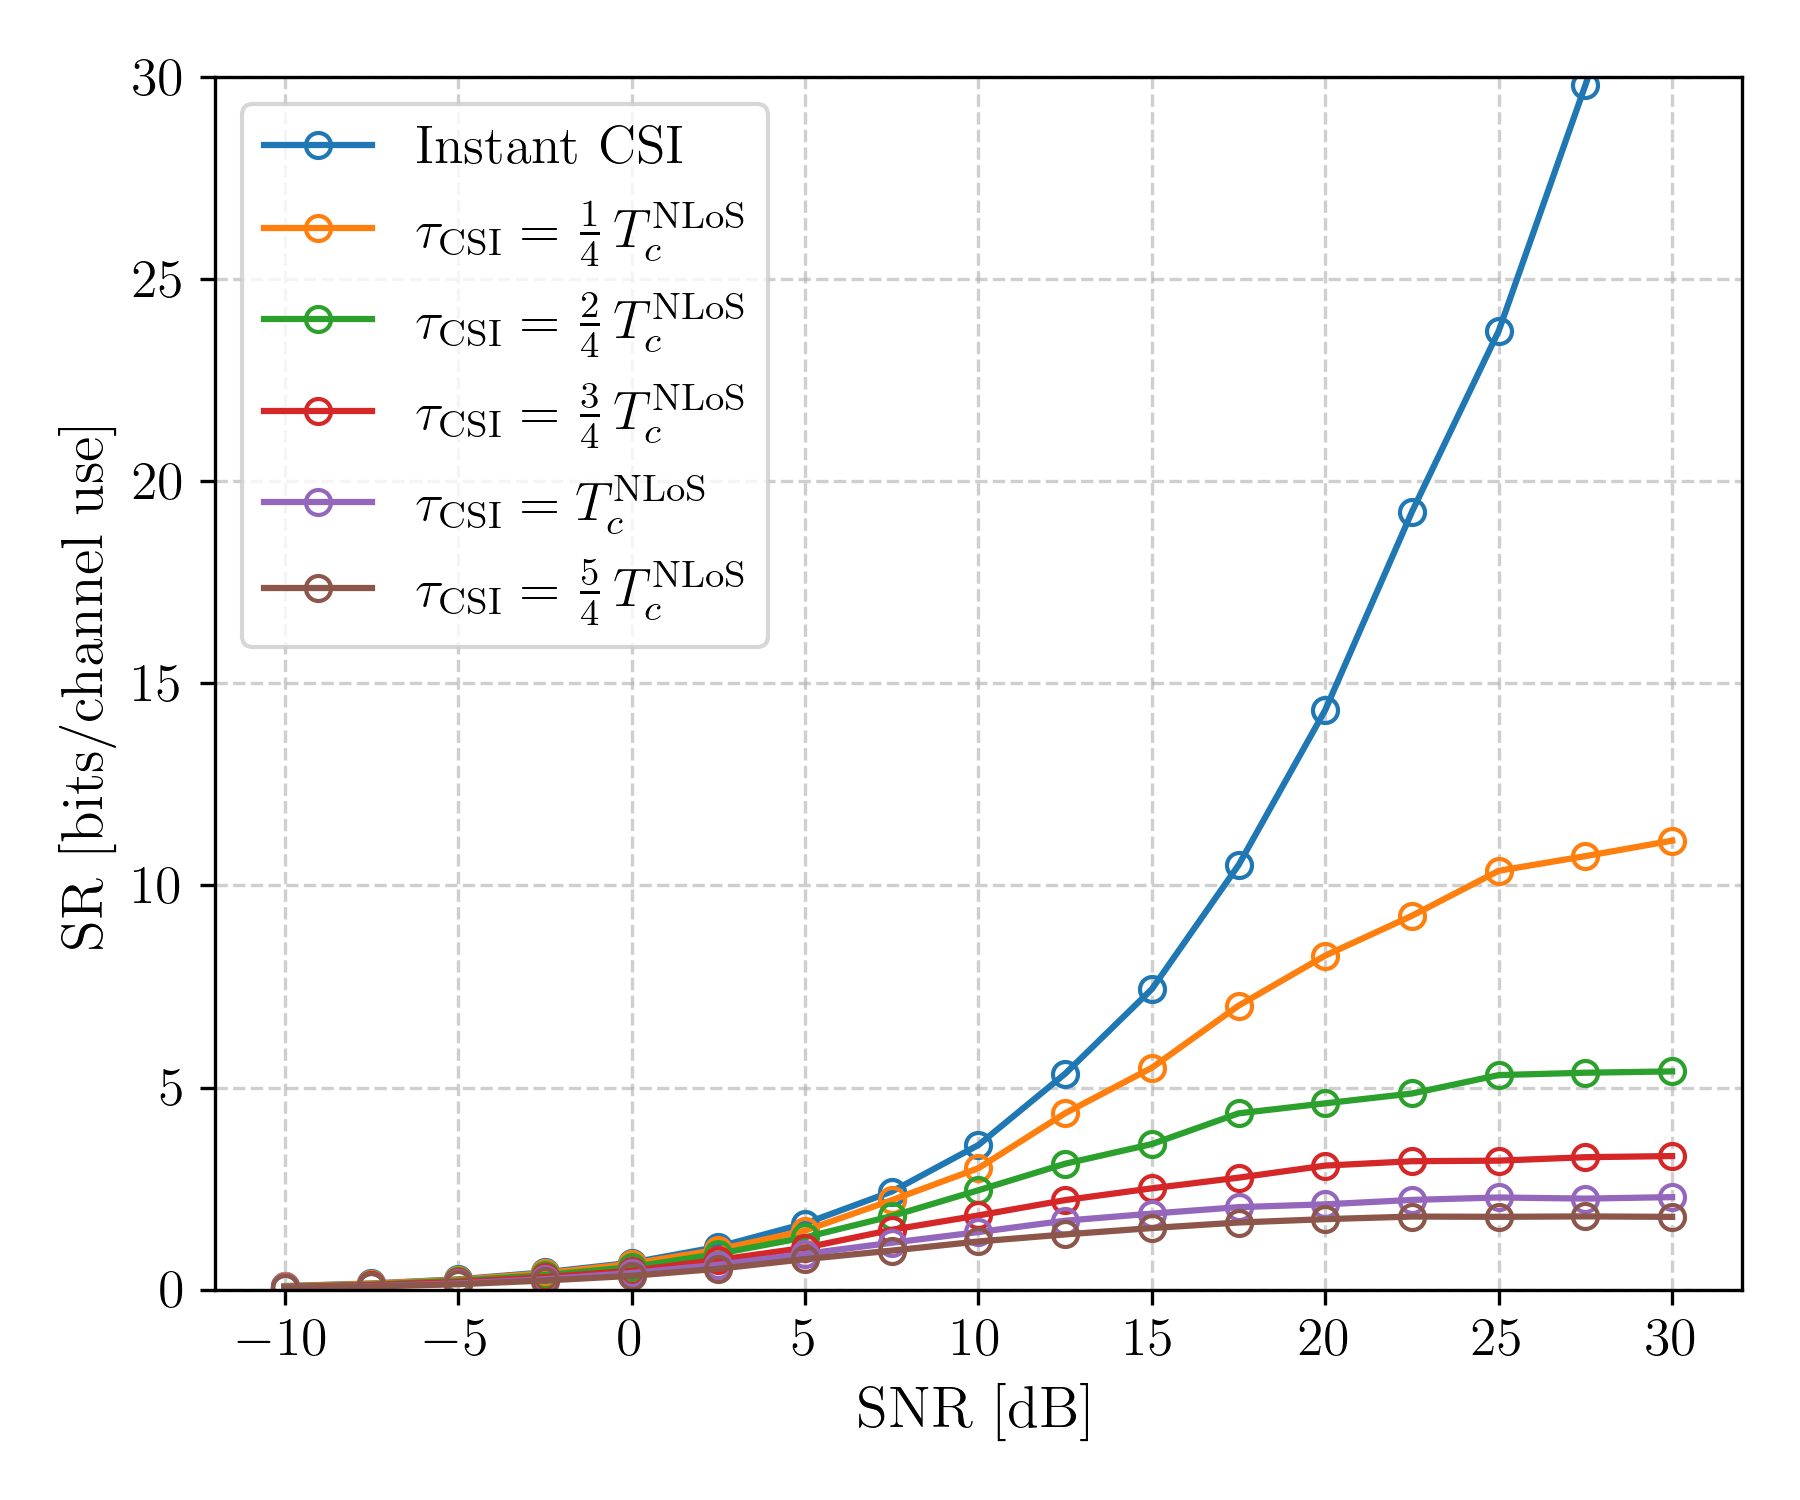
\includegraphics[width=\textwidth]{figures/mobile_satellite_systems/06_precoding_under_outdated_csi/rician_channel/impact_outdated_csi/achievable_rate_zf.png}
        \caption{\acs{ZF} Precoding}
        \label{fig:impact_outdated_csi_achievable_rate_zf}
    \end{subfigure}
    \hfill
    \begin{subfigure}{0.495\textwidth}
        \centering
        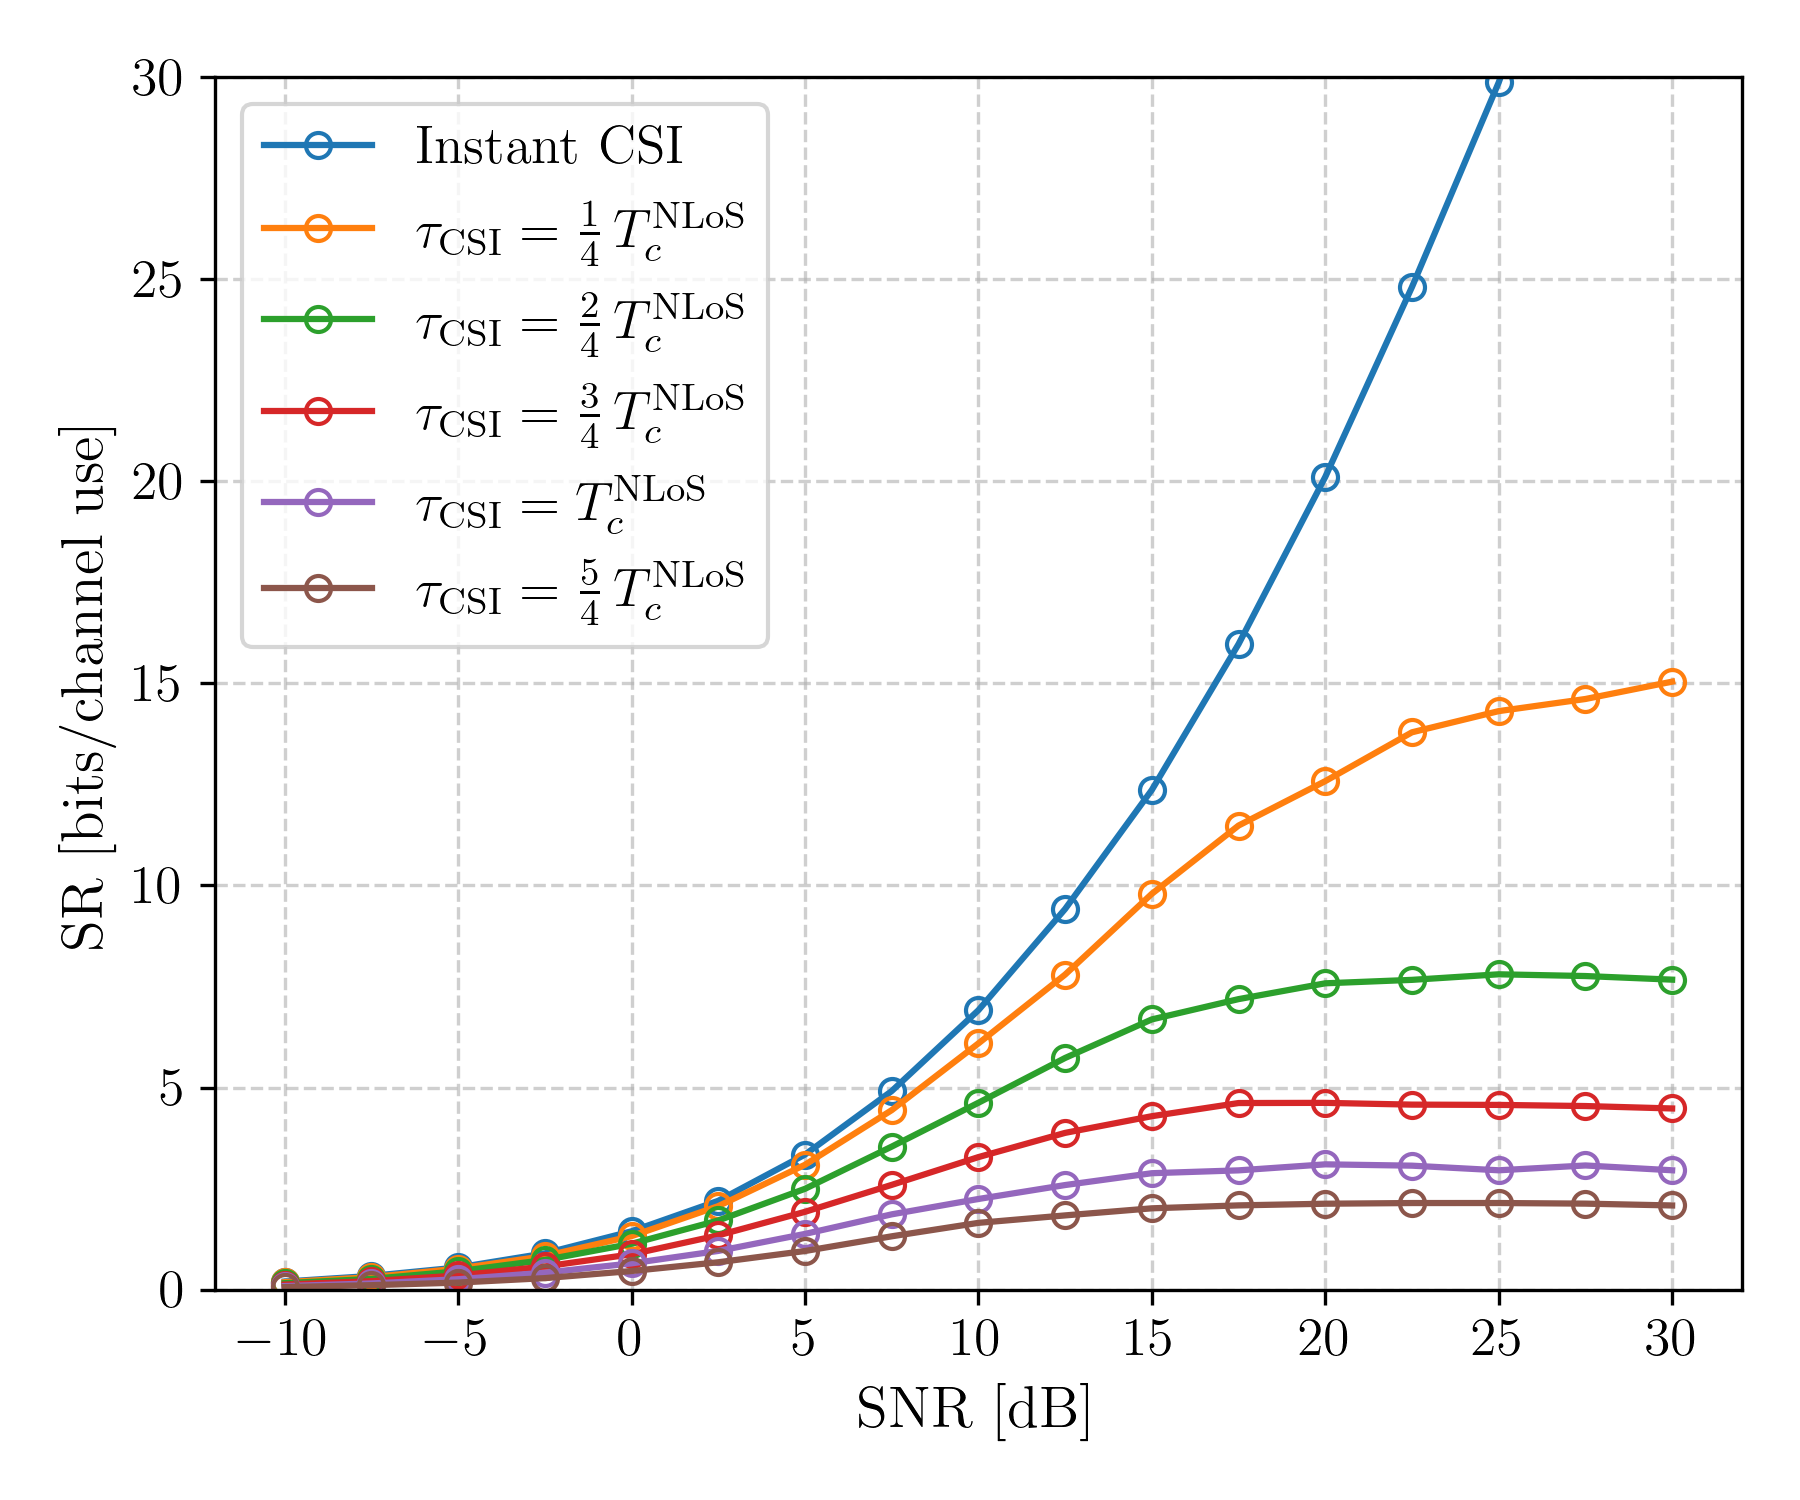
\includegraphics[width=\textwidth]{figures/mobile_satellite_systems/06_precoding_under_outdated_csi/rician_channel/impact_outdated_csi/achievable_rate_bd.png}
        \caption{\acs{BD} Precoding}
        \label{fig:impact_outdated_csi_achievable_rate_bd}
    \end{subfigure}
    \caption[Impact of outdated \acs{CSI} on the achievable sum-rate (\acs{ZF} and \acs{BD} precoding)]{
        The achievable sum-rate of a  $8 \times \{2, 2, 2, 2\} $ \acs{MU}-\acs{MIMO} system as a function of the \acs{SNR}, for \acs{ZF} and \acs{BD} precoding.
        The different curves correspond to different values of the \acs{CSI} feedback delay $\tau_{\mathrm{CSI}}$, expressed as a fraction of the coherence time $T_c$.
    }
    \label{fig:impact_outdated_csi_achievable_rate_zf_bd}
\end{figure}

% WMMSE
The \ac{WMMSE} precoder exhibits a qualitatively different behaviour.
The achievable rate reaches a maximum and decreases slightly beyond it when the precoder design relies on outdated \ac{CSI}, as is clearly visible in Figure~\ref{fig:impact_outdated_csi_achievable_rate_wmmse}.
Unlike \ac{ZF} and \ac{BD}, \ac{WMMSE} precoding adapts its solution to the operating \ac{SNR}.
At low \ac{SNR} it trades interference suppression against desired-signal power, while at high \ac{SNR} the regularization vanishes and it converges to the interference-free \ac{BD} solution.
The algorithm then increasingly concentrates power in directions that it expects to be beneficial, but which, due to the channel mismatch, actively generate inter-user interference in the actual channel.
The \ac{ZF}-type precoders do not exhibit this behaviour because they steer in the wrong direction just as aggressively for any \ac{SNR} value.

\begin{figure}[!htb]
    \centering
    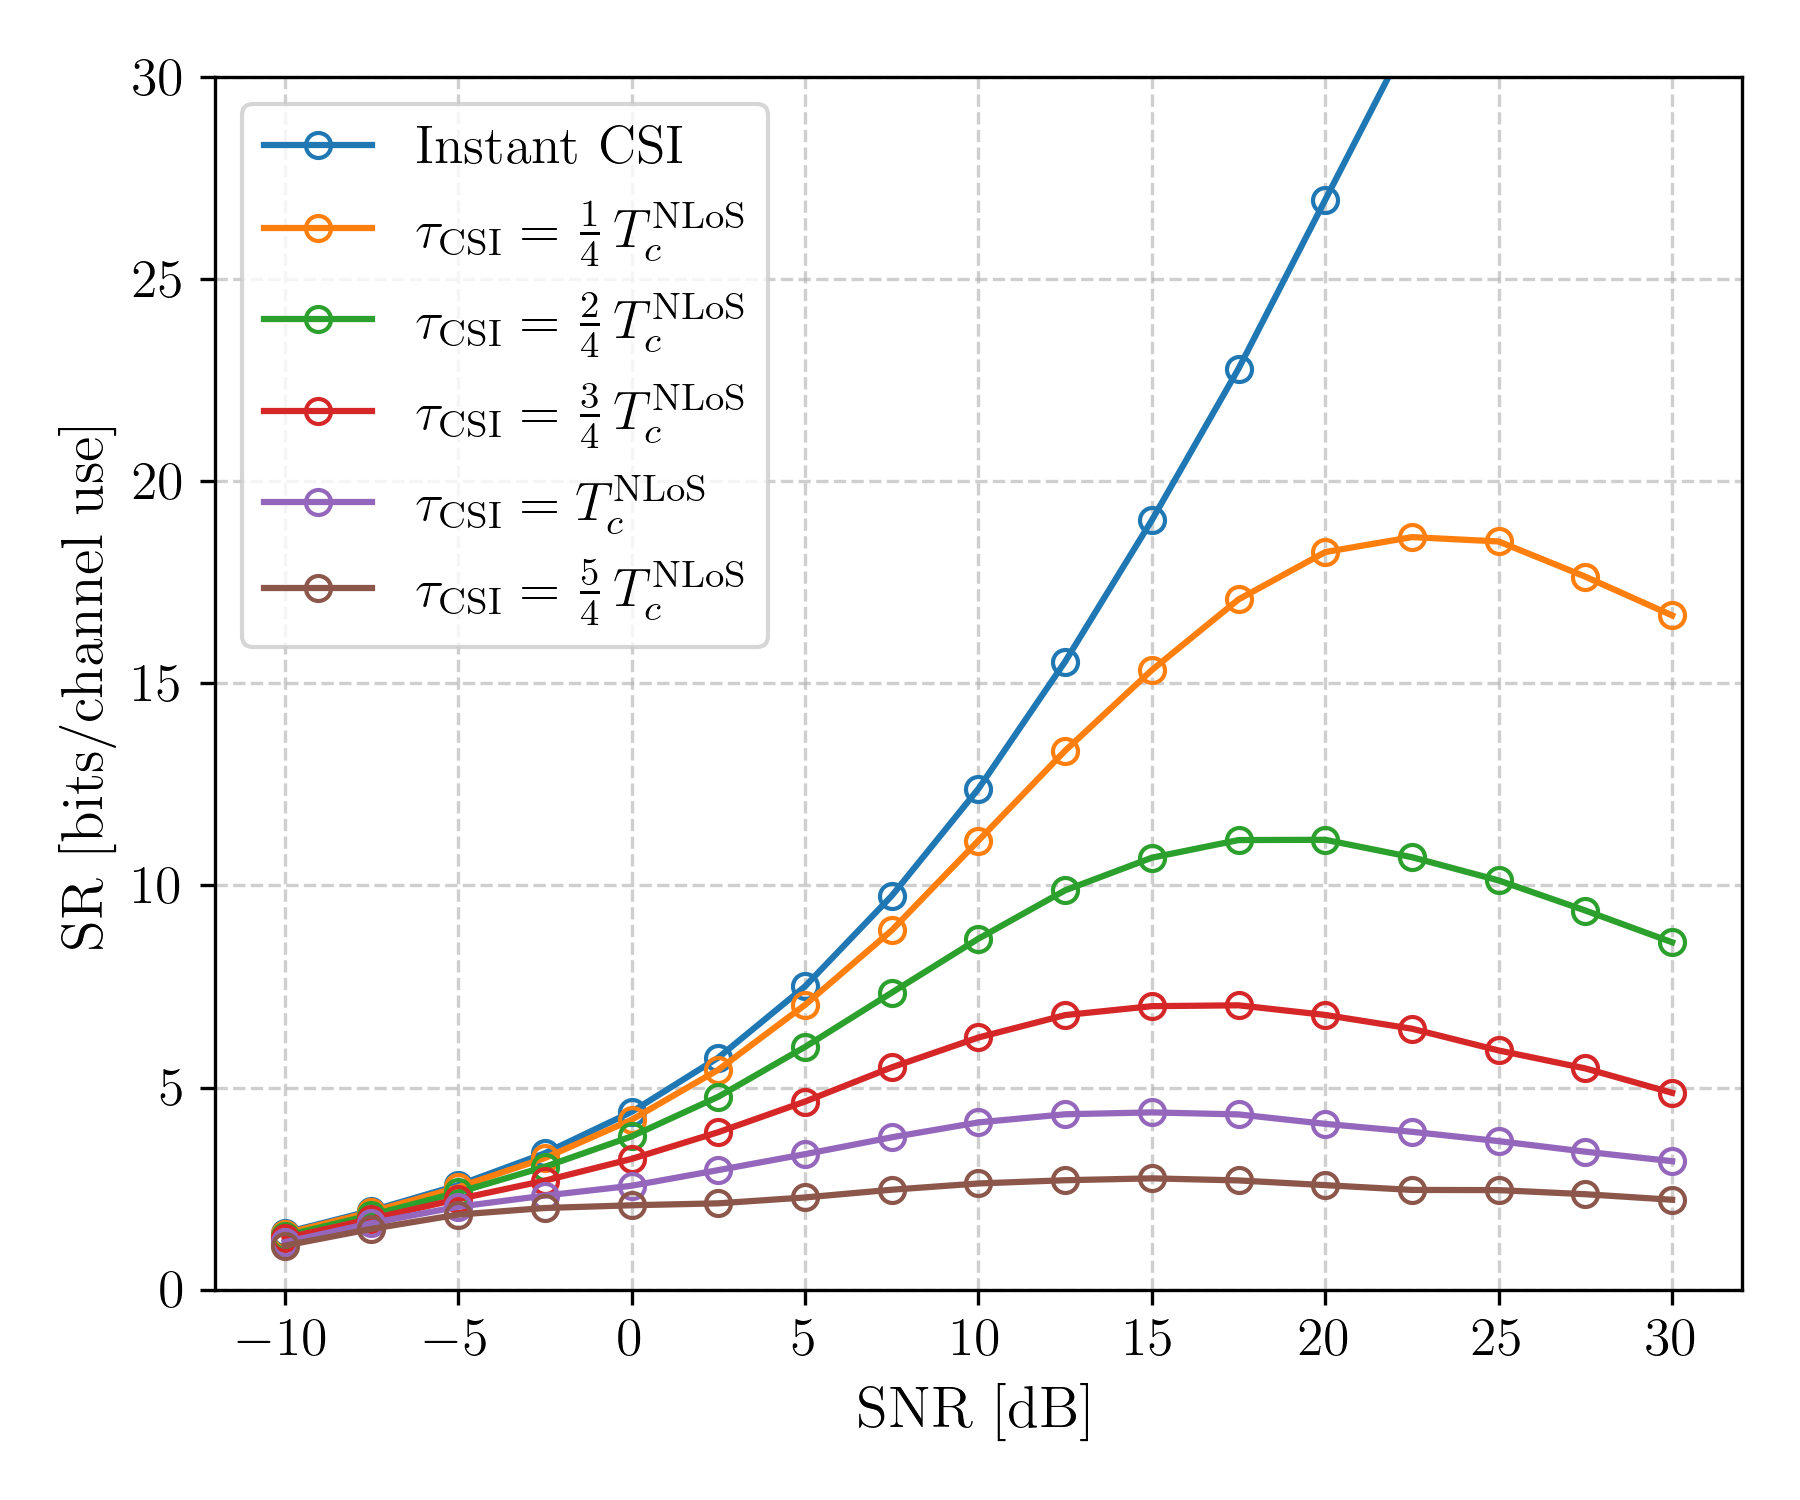
\includegraphics[width=0.65\textwidth]{figures/mobile_satellite_systems/06_precoding_under_outdated_csi/rician_channel/impact_outdated_csi/achievable_rate_wmmse.png}
    \caption[Impact of outdated \acs{CSI} on the achievable sum-rate (\acs{WMMSE} precoding)]{
        Similar figure as Fig.~\ref{fig:impact_outdated_csi_achievable_rate_zf_bd}, but for \acs{WMMSE} precoding.
    }
    \label{fig:impact_outdated_csi_achievable_rate_wmmse}
\end{figure}

% Rician vs Rayleigh
A final observation concerns the reference curve obtained with instantaneous \ac{CSI}.
Even in this idealised case, the achievable rate lies noticeably below the values obtained in Chapter~\ref{chapter:mu_mimo_precoding} under a purely Rayleigh fading channel.
This accounts for all three precoding techniques, and is a direct consequence of the \ac{LoS} contribution in a Rician channel.
Indeed, the \ac{LoS} component is rank-one, such that the largest fraction of the channel energy is concentrated along a single spatial direction.
A purely Rayleigh fading channel, by contrast, provides rich spatial diversity and a well-conditioned channel matrix, granting the precoder significantly more spatial multiplexing gain.
Therefore, the \ac{LoS} component imposes an inherent limit on the spatial degrees of freedom available, regardless of the quality of the \ac{CSI}.

% outro
Taken together, these results show that even a small feedback delay poses a threat to the achievable rate at moderate and high \ac{SNR}, and that no choice of precoder can restore the linear growth observed with instantaneous \ac{CSI} by itself.
The next section therefore turns to the design of a compensation strategy that targets the source of the problem, which is the temporal mismatch between $\mathbf{H}(t - \tau_{\mathrm{CSI}})$ and $\mathbf{H}(t)$, rather than its consequences.

\section{Compensation for Outdated CSI}
\label{section:outdated_csi_compensation}
% =====================================
%    Compensation for Outdated CSI
% =====================================

As established in the previous section, the degradation observed in Section~\ref{section:outdated_csi_impact} stems from the mismatch between the channel estimate available at the \ac{GW} and the channel experienced at the time of transmission.
However, the channel is a temporally correlated random process, and the history of past channel estimates therefore carries useful information about the current channel state.
In what follows, we propose a simple compensation strategy that exploits the temporal correlation to predict, at each \ac{UT}, the channel that will be experienced after the \ac{CSI} feedback delay, and feed this predicted channel back to the \ac{GW} instead of the most recent channel estimate.
The performance gain introduced by this strategy will again be evaluated by means of a simulation.

\subsection{Compensation Strategy}
\label{subsection:compensation_strategy}
% ----------------------------------

% strategy philosophy: AR-model
Among the many possible prediction methods, a linear \acf{AR} model is adopted here as a simple and tractable baseline. It leads to a closed-form predictor, requires only knowledge of the autocorrelation function, and entails a very limited computational complexity.
The prediction is performed locally at each \ac{UT}, while the \ac{GW} continues to compute the precoder exactly as in Chapter~\ref{chapter:mu_mimo_precoding}. From the perspective of the \ac{GW}, the precoding procedure is therefore unchanged. Only the channel information on which it relies is replaced by a prediction of the future channel state. As a result, the additional complexity introduced by the compensation strategy is borne entirely by the \acp{UT}.

% AR-model mechanism
Under the simplified channel model of Chapter~\ref{chapter:hts_communication_systems}, the temporal variation is entirely contained in the \ac{NLoS} component. Moreover, spatial correlation within the \ac{NLoS} component is neglected, so that the entries of $\mathbf{H}_k^{\mathrm{NLoS}}(t)$ evolve independently and share the same temporal correlation function. Therefore, we choose to carry out the prediction element-wise, using the same scalar predictor for each channel coefficient. 
Let $\hat{h}_{k, \,(i, j)}[n]$ denote the estimate of the $(i,j)$-th entry of the channel matrix of \ac{UT}~$k$ at the $n$-th pilot instant. A $p$-th order \ac{AR} predictor of the channel $\Delta$ pilot intervals ahead is then written as
\begin{equation}
\label{eq:ar_predictor}
    \hat{h}_{k, \,(i, j)}[n+\Delta] = \sum_{m=0}^{p-1} \alpha_m \, \hat{h}_{k, \,(i, j)}[n-m].
\end{equation}
The prediction horizon $\Delta$ is chosen such that the predicted sample corresponds to the actual transmission time, that is, $\Delta \, T_p = \tau_{\mathrm{CSI}}$, where $T_p$ denotes the pilot period.

The predictor coefficients $\{\alpha_m\}_{m=1}^{p}$ are obtained from the Yule--Walker equations associated with the autocorrelation function $R_h(\tau)$ of the channel process:
\begin{equation}
\label{eq:yule_walker_equations}
    \begin{bmatrix} R_h(0) & R_h(T_p) & \cdots & R_h((p-1)T_p) \\ R_h(T_p) & R_h(0) & \cdots & R_h((p-2)T_p) \\ \vdots & \vdots & \ddots & \vdots \\ R_h((p-1)T_p) & R_h((p-2)T_p) & \cdots & R_h(0) \end{bmatrix} \; \begin{bmatrix} \alpha_1 \\ \alpha_2 \\ \vdots \\ \alpha_p \end{bmatrix} = \begin{bmatrix} R_h(\Delta T_p) \\ R_h((\Delta+1)T_p) \\ \vdots \\ R_h((\Delta+p-1)T_p) \end{bmatrix}.
\end{equation}
Since the autocorrelation function is fully specified by the assumed channel model, these coefficients can be computed offline once the predictor order $p$, the pilot period $T_p$, and the delay $\tau_{\mathrm{CSI}}$ have been fixed.

% assumptions
Three assumptions underlie the proposed compensation strategy.
First, channel-estimation errors are neglected, so that the channel estimates available at the \acp{UT} are assumed to be perfect.
Second, each \ac{UT} is assumed to know the second-order statistics of its channel. In the present model, this amounts to knowing the autocorrelation function $R_h(\tau)$, which under Jakes' model is fully determined by the maximum Doppler frequency $f_D$. This is a reasonable assumption, since $f_D$ can be estimated locally from the carrier frequency and the \ac{UT} velocity.
Third, the pilot period $T_p$ is treated as a free design parameter and is not constrained by a pilot-overhead budget. This idealization makes it possible to characterize the intrinsic potential of the compensation strategy independently of the resource limitations of a specific system implementation.

\subsection{Parameter Optimization}
\label{subsection:compensation_parameter_optimization}
% ----------------------------------------------------

% two free parameters
The predictor of~\eqref{eq:ar_predictor} is controlled by two free parameters. 
First, the pilot period $T_p$, or equivalently the pilot rate $1/T_p$, which determines the temporal resolution at which the channel is observed.
Second, the time span or context window length $L \triangleq p\, T_p$ covered by the $p$ past samples, which controls how far back in time the predictor reaches.
For a fixed window length, a higher pilot rate raises the model order $p$ by providing finer temporal resolution, while for a fixed pilot rate, a longer window increases the model
order by incorporating older observations.
The order $p$ of the \ac{AR} model is fixed once $T_p$ and $L$ are chosen through the relation $p = L/T_p$, and thus not considered as a third design parameter.
Both model parameters are expressed relative to the coherence time of the channel, in line with the normalization of the \ac{CSI} feedback delay adopted throughout this chapter.

% decoupled optimization
Rather than performing a joint grid search over $T_p$ and $L$, the two parameters are tuned sequentially. 
The pilot rate is first optimized with the context window length held fixed at a conservative value, after which the context window length is tuned with the pilot rate frozen at the value found in the first step.
Both optimisations are evaluated for the $8 \times \{2, 2, 2, 2\}$ system using \ac{WMMSE} precoding at a single operating point with an \ac{SNR} equal to $20~\mathrm{dB}$, for different values of \ac{CSI} feedback delay.

\begin{figure}[!b]
    \centering
    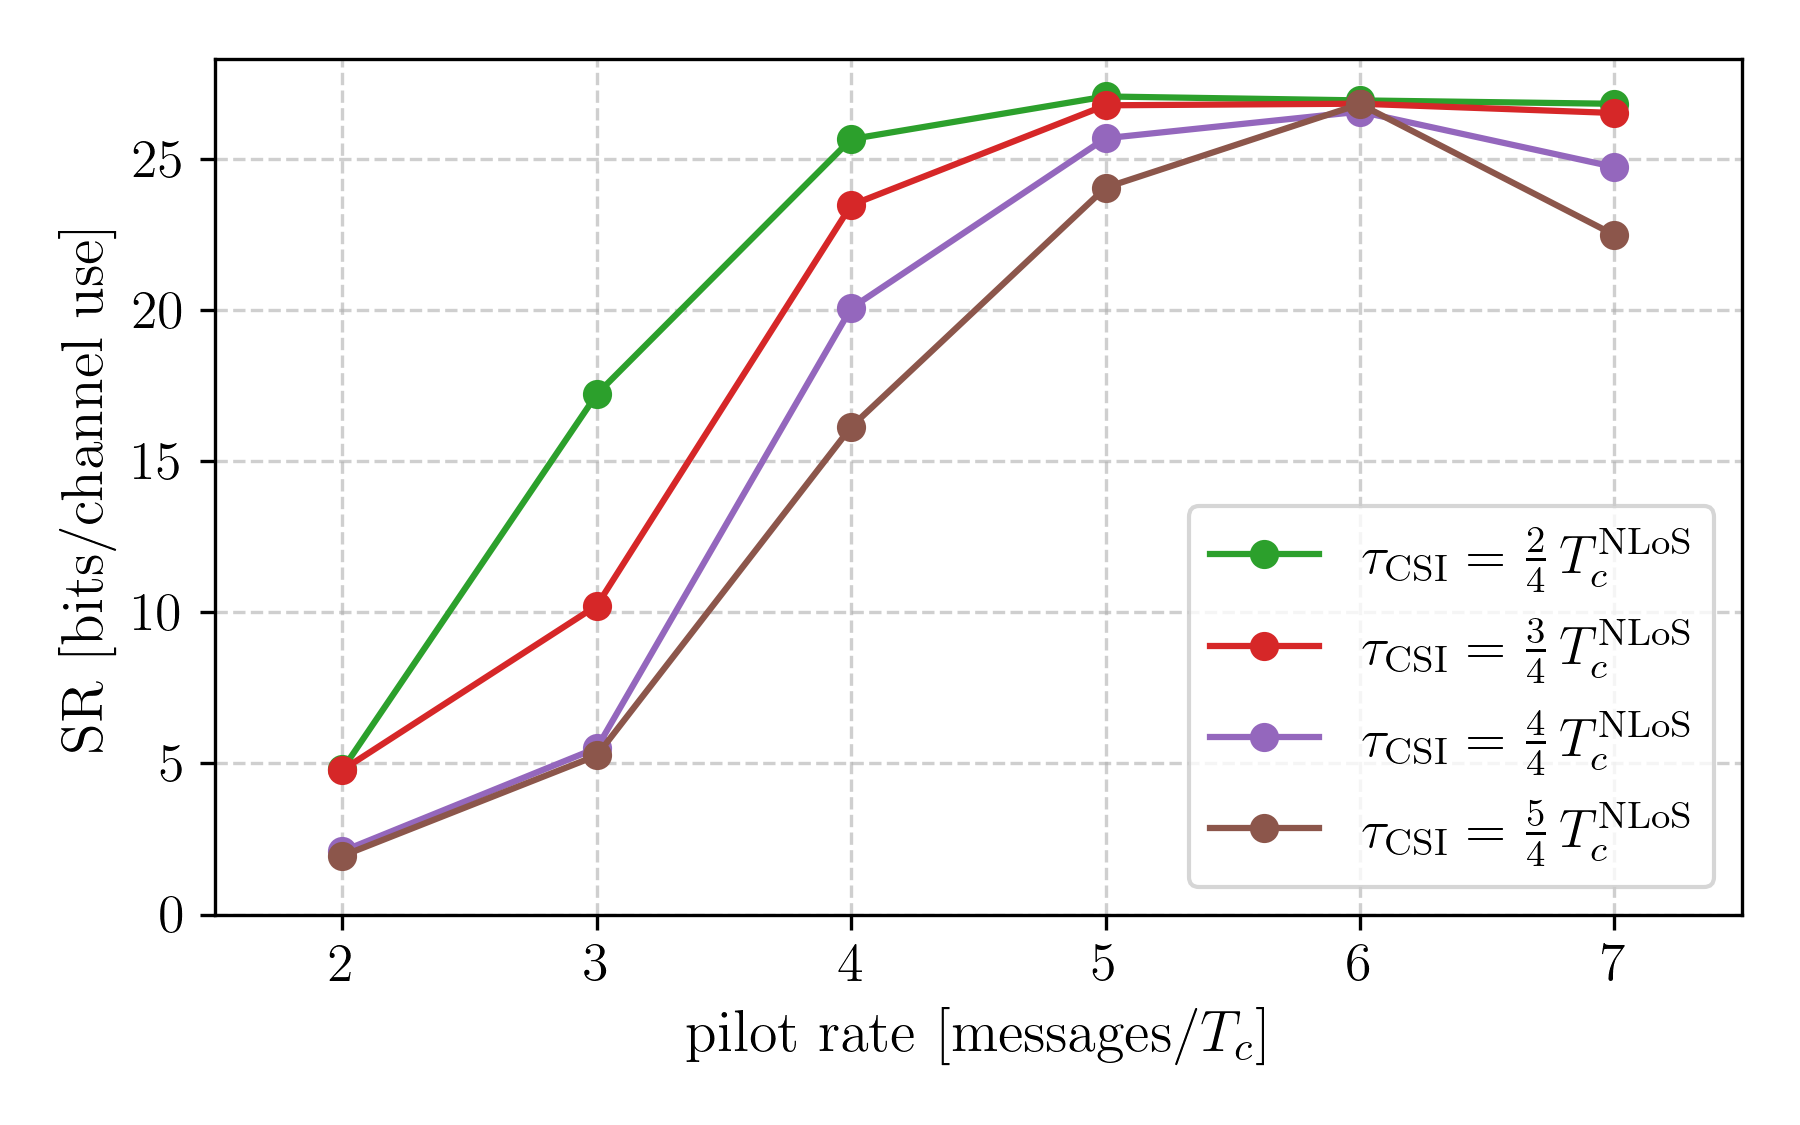
\includegraphics[width=0.65\textwidth]{figures/mobile_satellite_systems/06_precoding_under_outdated_csi/rician_channel/ar_model_parameter_choice/pilot_rate_wmmse.png}
    \caption[Impact of the pilot rate on the achievable sum-rate with \acs{AR}-based compensation]{
        The achievable sum-rate plotted as a function of the pilot rate.
        The $8 \times \{2, 2, 2, 2\}$ system uses a \acs{WMMSE} precoder and \acs{AR}-based channel prediction model at the \acs{UT}, and operates at a \ac{SNR} equal to $20~\mathrm{dB}$.
        The context window length is fixed to $2\,T_c$.
        Each curve corresponds to a different \acs{CSI} feedback delay.
    }
    \label{fig:parameter_pilot_rate}
\end{figure}

% pilot rate
For the first sweep, the context window length fixed at $2\,T_c$. This is a generous choice, made to ensure that no potentially useful information would be excluded.
Figure~\ref{fig:parameter_pilot_rate} shows the achievable sum-rate as a function of the pilot rate for four values of the \ac{CSI} feedback delay.
The achievable sum-rate increases steadily as the pilot rate grows, reflecting the improvement in temporal resolution available to the predictor. 
When too few samples are available within the temporal correlation window to capture the channel dynamics accurately, the achievable sum-rate drops rapidly, especially for the larger feedback delays.
At $6$ messages per $T_c$, all four curves reach their respective maximum and converge to nearly the same value, indicating that the compensation is equally effective regardless of the feedback delay.
Increasing the pilot rate further than $6$ messages per coherence time does not improve performance and even causes a slight degradation for the larger delays, most likely because the resulting high model order renders the Yule-Walker system ill-conditioned. The autocorrelation matrix then becomes increasingly close to singular.
A pilot rate of $6$ messages per coherence time is therefore selected.

% context window length
With the pilot rate fixed at $6$ messages per $T_c$, the context window length is varied.
Figure~\ref{fig:parameter_context_window_length_wmmse} shows that a too short window prevents the predictor from accessing enough of the temporal correlation of the channel and, as expected, severely degrades the achievable sum-rate.
Also, the curves saturate beyond a certain prediction horizon.
This aligns with the intuition that, after a certain point, the channel history is no longer significantly correlated with the value being predicted, such that the additional information contained in older samples is negligible.
This saturation point depends strongly on the \ac{CSI} feedback delay: for shorter feedback delays, a shorter window length suffices.
Note that a longer context window length results in a larger memory footprint at the \ac{UT}.
A context window length of one coherence period is therefore adopted for all subsequent simulations.

\begin{figure}[!htb]
    \centering
    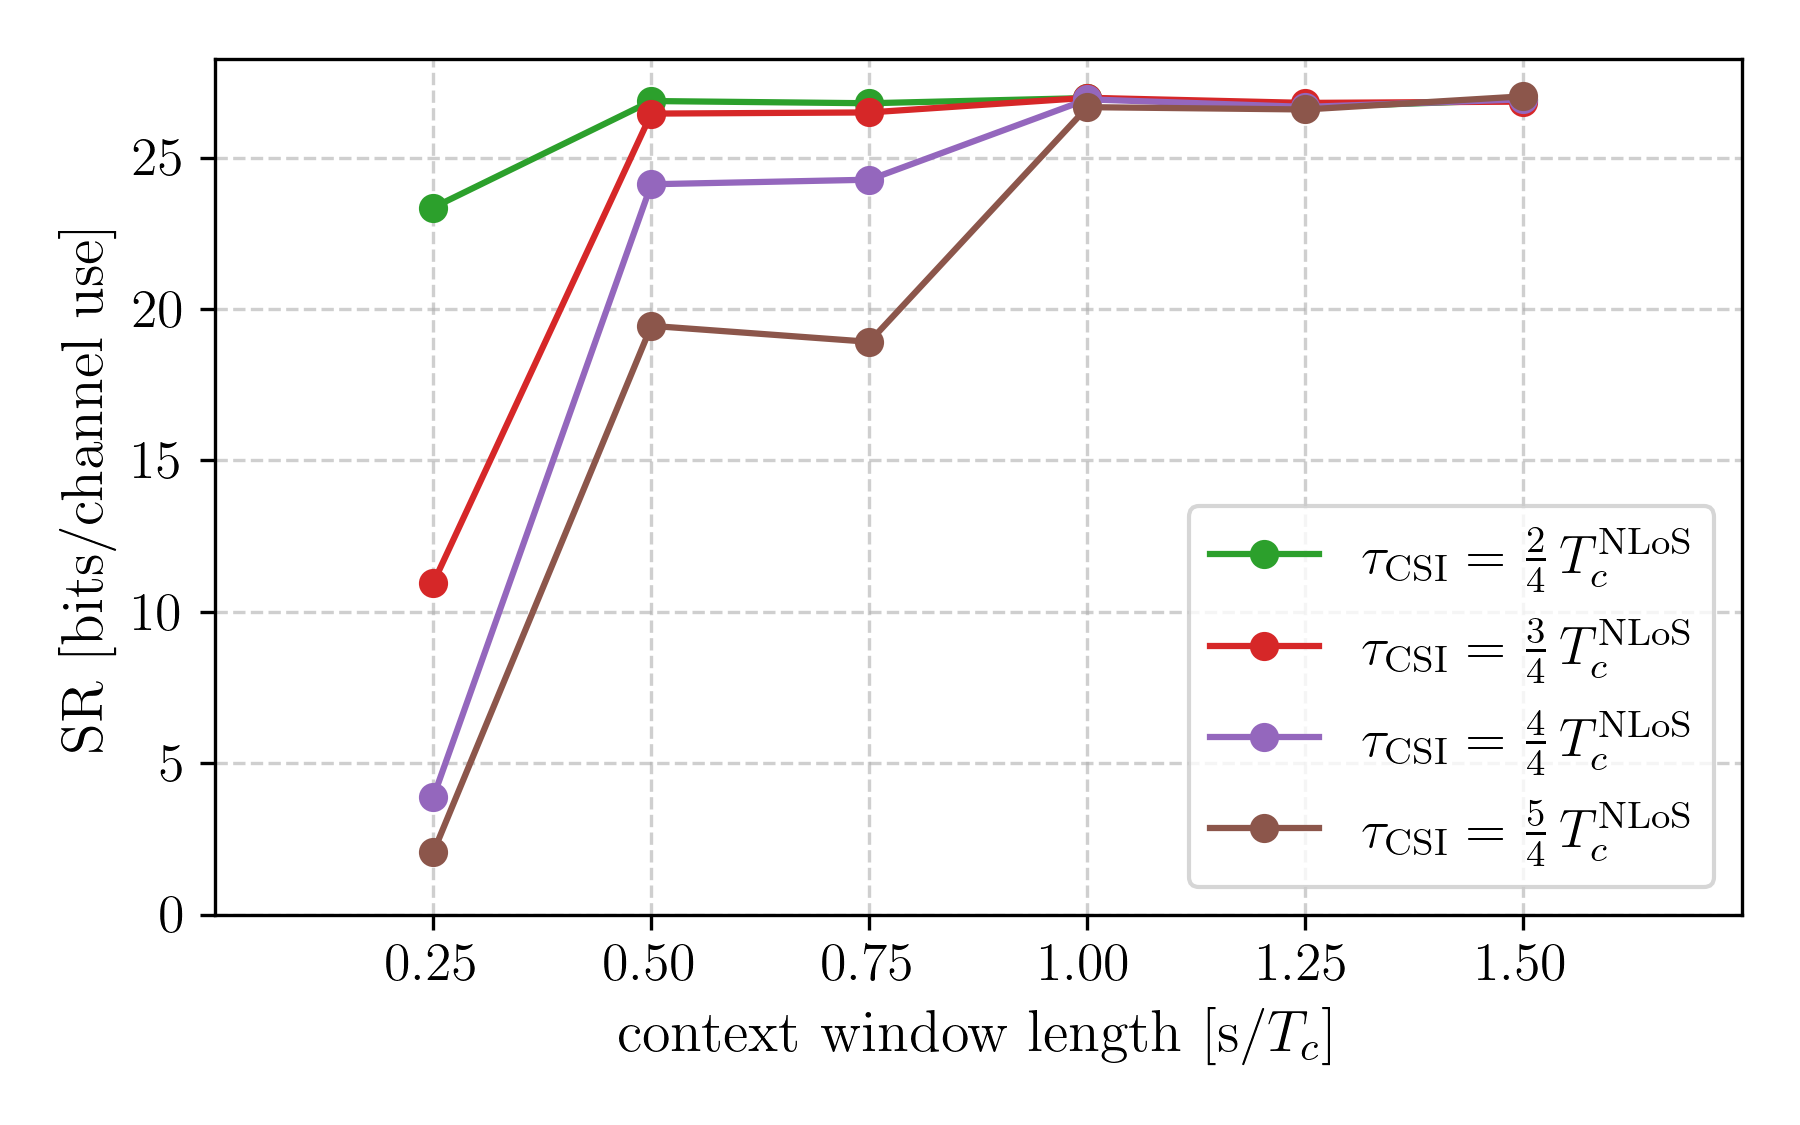
\includegraphics[width=0.65\textwidth]{figures/mobile_satellite_systems/06_precoding_under_outdated_csi/rician_channel/ar_model_parameter_choice/context_window_length_wmmse.png}
    \caption[Impact of the window length on the achievable sum-rate with \acs{AR}-based compensation]{
        The achievable sum-rate plotted as a function of the context window length.
        The pilot rate is set to $6$ messages per coherence period. 
        Other than that, the system operates under the exact same configurations in Fig.~\ref{fig:parameter_pilot_rate}.
    }
    \label{fig:parameter_context_window_length_wmmse}
\end{figure}

% outro
% In the remainder of this chapter, the compensation strategy is systematically evaluated using a predictor of order $6$, with samples uniformly distributed over a time interval equal to the channel coherence period.

\subsection{Performance Evaluation}
\label{subsection:compensation_performance_evaluation}
% ----------------------------------------------------

% intro
This subsection quantifies the gain achieved by the proposed \ac{AR}-based compensation strategy.
The predictor settings are those selected in Section~\ref{subsection:compensation_parameter_optimization}: a pilot rate of $6$ messages per coherence period and a context window length equal to one coherence period.
All other system configurations are kept identical to Section~\ref{section:outdated_csi_impact}, so that the effect of compensation can be isolated directly.
Figure~\ref{fig:impact_compensation_achievable_rate_zf_bd} shows the achievable sum-rate for \ac{ZF} and \ac{BD} precoding, and Figure~\ref{fig:impact_compensation_achievable_rate_wmmse} provides an explicit three-way comparison for \ac{WMMSE} precoding. Each panel shows the achievable sum-rate under perfect \ac{CSI}, outdated \ac{CSI}, and predicted \ac{CSI} for a single feedback delay.

\begin{figure}[!htb]
    \centering
    \begin{subfigure}{0.495\textwidth}
        \centering
        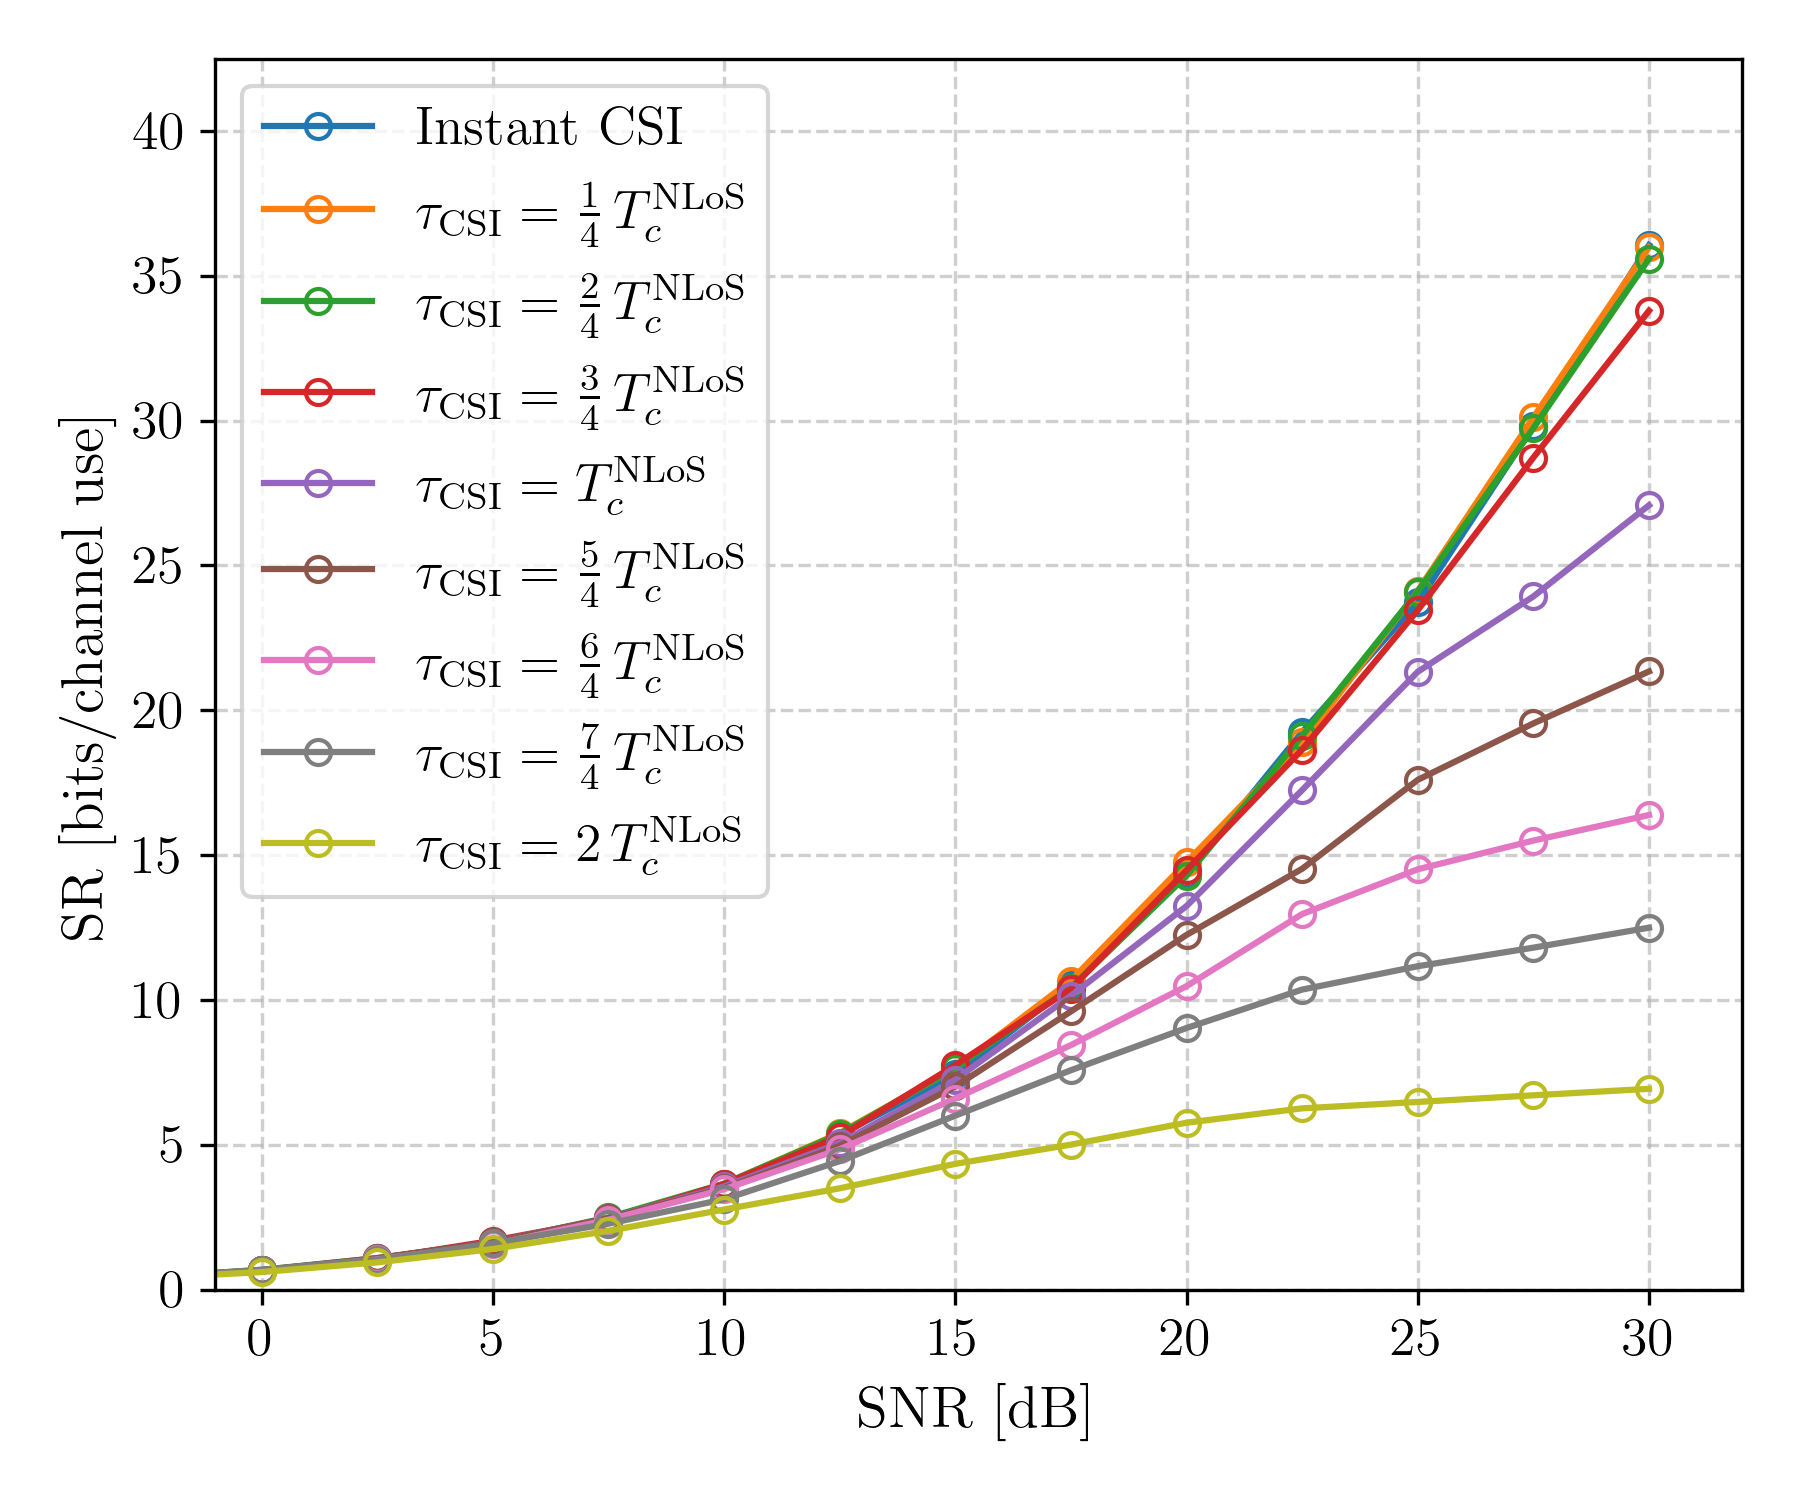
\includegraphics[width=\textwidth]{figures/mobile_satellite_systems/06_precoding_under_outdated_csi/rician_channel/impact_compensation/achievable_rate_zf.png}
        \caption{\acs{ZF} Precoding}
        \label{fig:impact_compensation_achievable_rate_zf}
    \end{subfigure}
    \hfill
    \begin{subfigure}{0.495\textwidth}
        \centering
        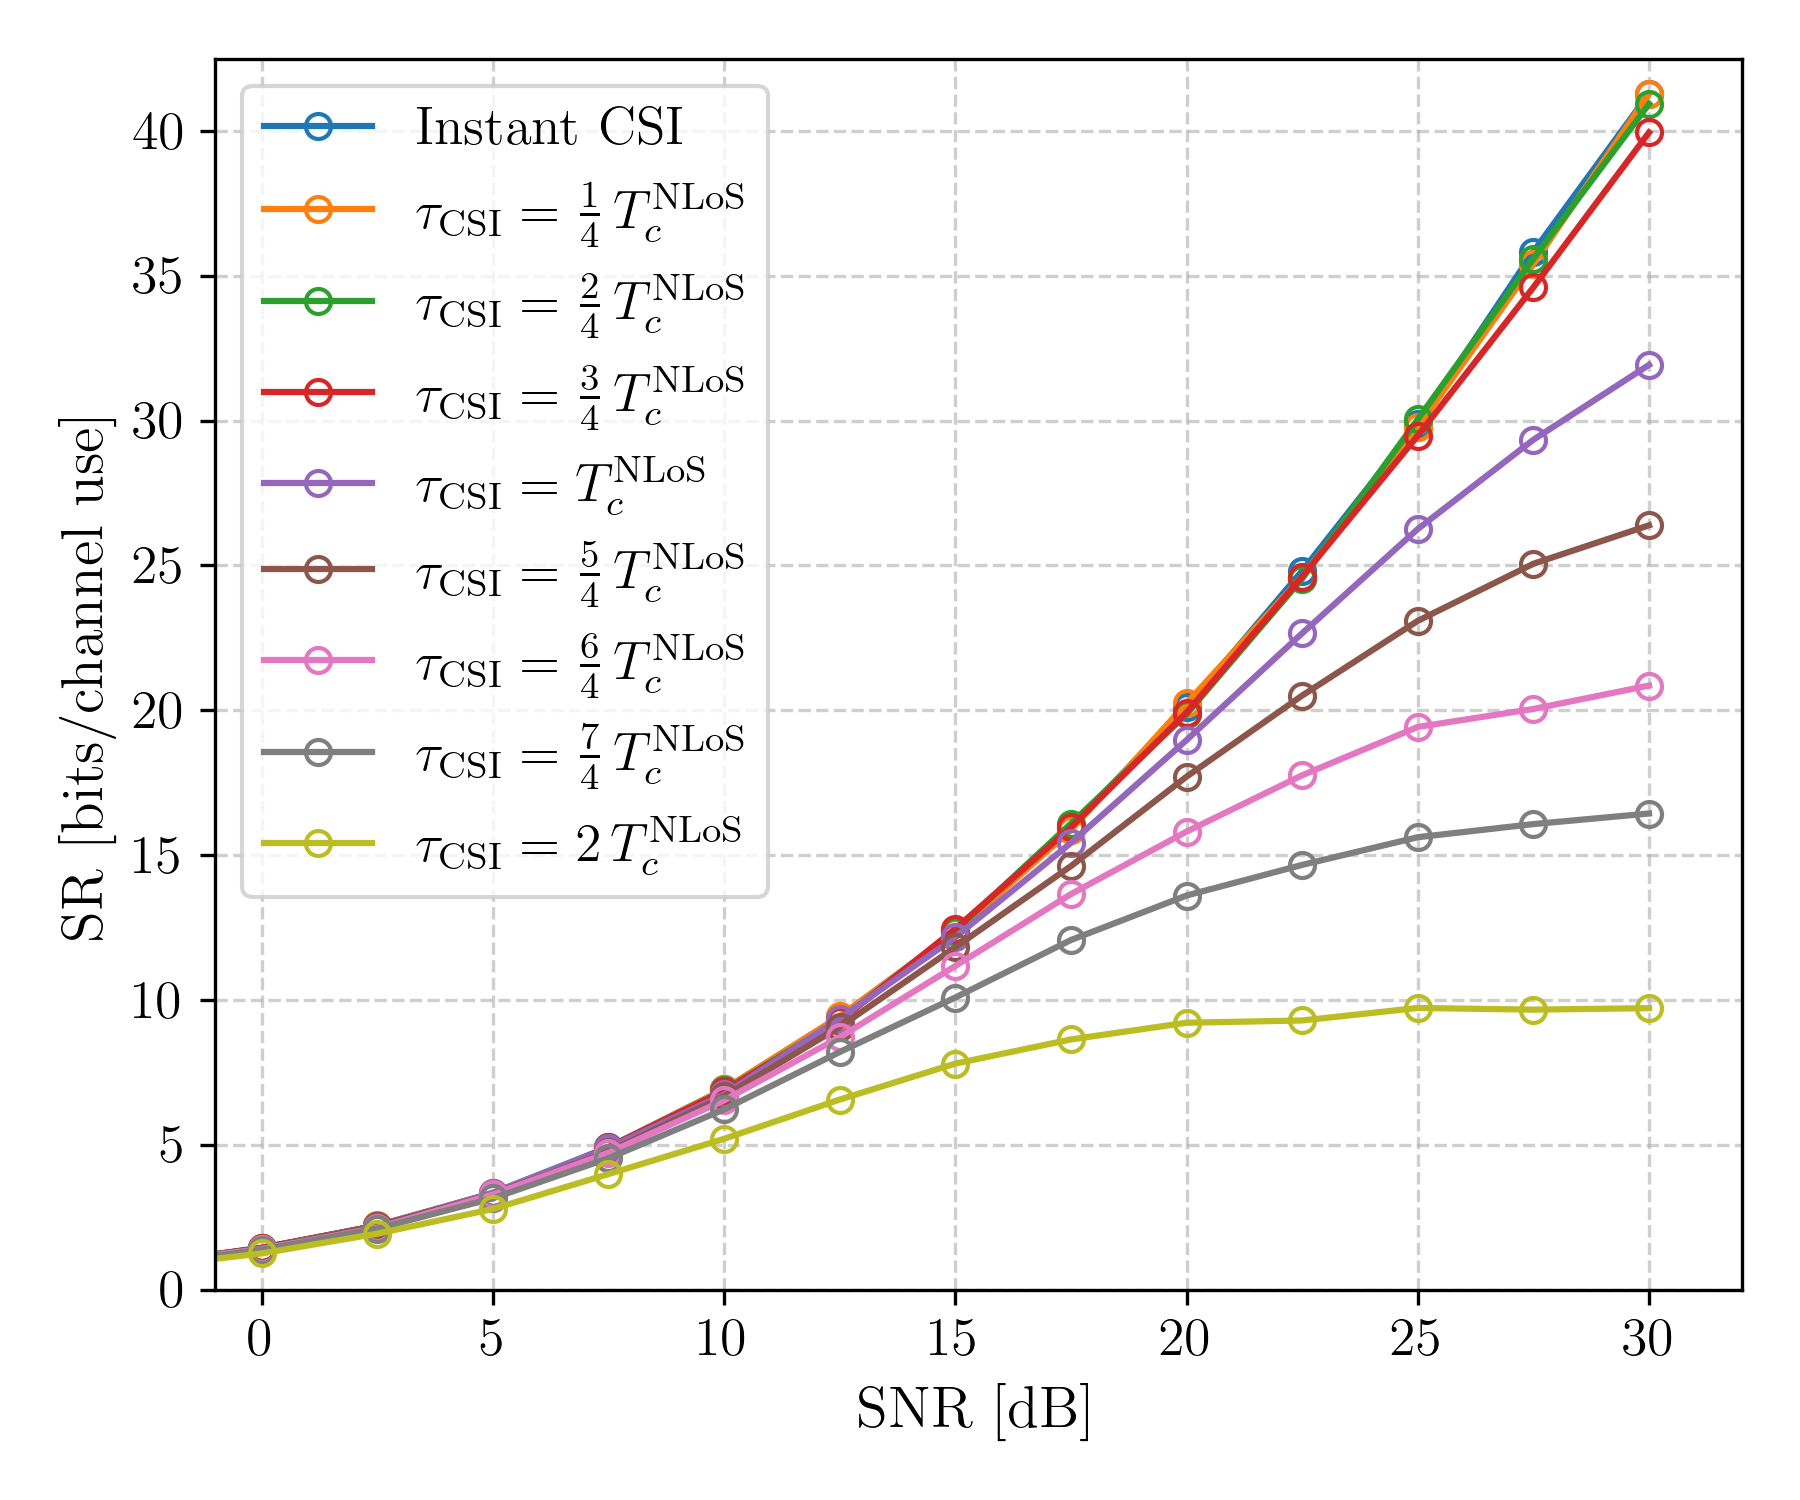
\includegraphics[width=\textwidth]{figures/mobile_satellite_systems/06_precoding_under_outdated_csi/rician_channel/impact_compensation/achievable_rate_bd.png}
        \caption{\acs{BD} Precoding}
        \label{fig:impact_compensation_achievable_rate_bd}
    \end{subfigure}
    \caption[Impact of the proposed compensation technique on achievable sum-rate (\acs{ZF} and \acs{BD})]{
        The achievable sum-rate as a function of the \acs{SNR} for \acs{ZF} and \acs{BD} precoding with \acs{AR}-based channel prediction at the \acp{UT}. 
        The predictor uses the parameter pair selected in Section~\ref{subsection:compensation_parameter_optimization}.
        The different curves correspond to different \acs{CSI} feedback delays, from no delay up to a delay equal to $2$ coherence periods of the \acs{NLoS} component.
    }
    \label{fig:impact_compensation_achievable_rate_zf_bd}
\end{figure}

% general observations
Figures~\ref{fig:impact_compensation_achievable_rate_zf_bd} and~\ref{fig:impact_compensation_achievable_rate_wmmse} show a consistent trend across all three precoding techniques.
For feedback delays up to approximately one coherence time, the compensation mechanism restores the performance obtained with instantaneous \ac{CSI} almost completely.
This confirms that the dominant part of the mismatch can be mitigated as long as the predictor operates within a time interval where the \ac{NLoS} component remains sufficiently correlated.
When the feedback delay exceeds the coherence time, the gain gradually decreases.
This behaviour is expected: for $\tau_{\mathrm{CSI}} > T_c$, the channel samples available to the predictor become weakly correlated with the target value, so the predicted channel cannot accurately track the channel realization experienced at the time of transmission.
The compensation strategy remains beneficial in this regime, but the residual mismatch grows with delay and the achievable sum-rate drops accordingly.

% disappearance of ceiling / peak-and-decrease
A remarkable difference between Figure~\ref{fig:impact_outdated_csi_achievable_rate_zf_bd} and Figures~\ref{fig:impact_compensation_achievable_rate_zf_bd} is the disappearance of the rate ceiling.
The compensation strategy restores the growth of the achievable sum-rate with increasing \ac{SNR} for almost all considered \ac{CSI} feedback delays.
Only when $\tau_{\mathrm{CSI}}$ approaches $2\,T_c$, the residual prediction error is large enough to reintroduce an interference floor, and the familiar saturation behaviour of §\ref{section:outdated_csi_impact} reappears.
A similar observation can be made for \ac{WMMSE} precoding.
Only for feedback delays well above $T_c$, the sum-rate exhibits the peak-and-decrease behaviour identified in Section~\ref{section:outdated_csi_impact}.

% conclusion
Altogether, these results show that channel prediction at the \acp{UT} is an effective and low-complexity mitigation mechanism for \ac{CSI} aging under the Rician fading channel model.
The largest performance gains are obtained when the feedback delay is on the order of, or smaller than, the coherence time of the \ac{NLoS} component.

\begin{figure}[!ht]
    \centering

    \makebox[\textwidth][c]{%
        \begin{minipage}{1.2\textwidth}
            \centering

            % First row
            \begin{subfigure}{0.245\textwidth}
                \centering
                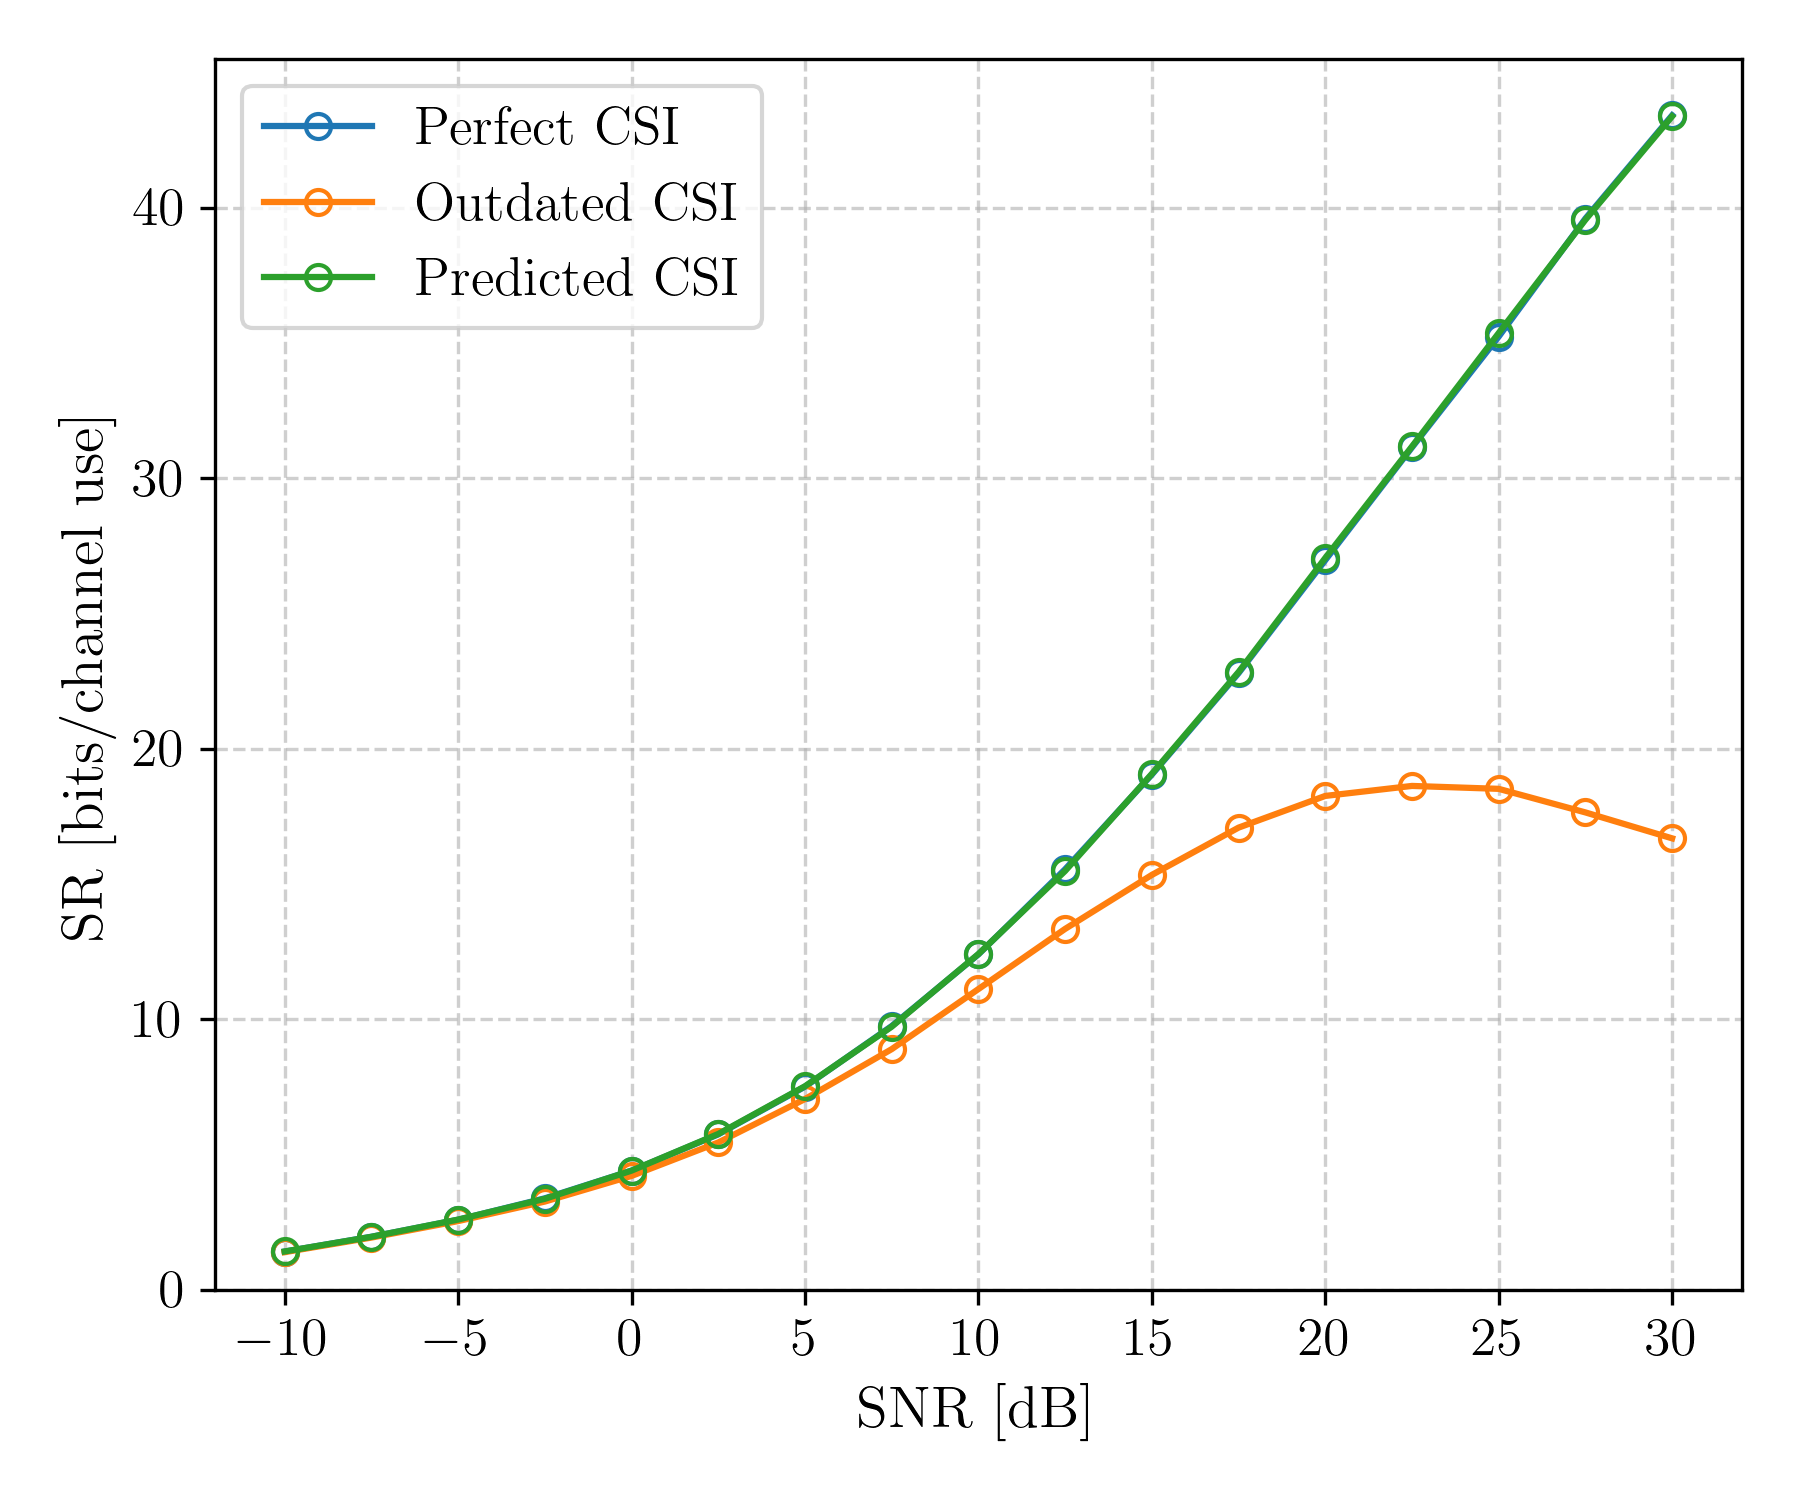
\includegraphics[width=\textwidth]{figures/mobile_satellite_systems/06_precoding_under_outdated_csi/rician_channel/impact_compensation/comparisons/wmmse/1on4.png}
                \caption{$\tau_{\mathrm{CSI}} = \frac{1}{4} T_c$}
            \end{subfigure}
            \hfill
            \begin{subfigure}{0.245\textwidth}
                \centering
                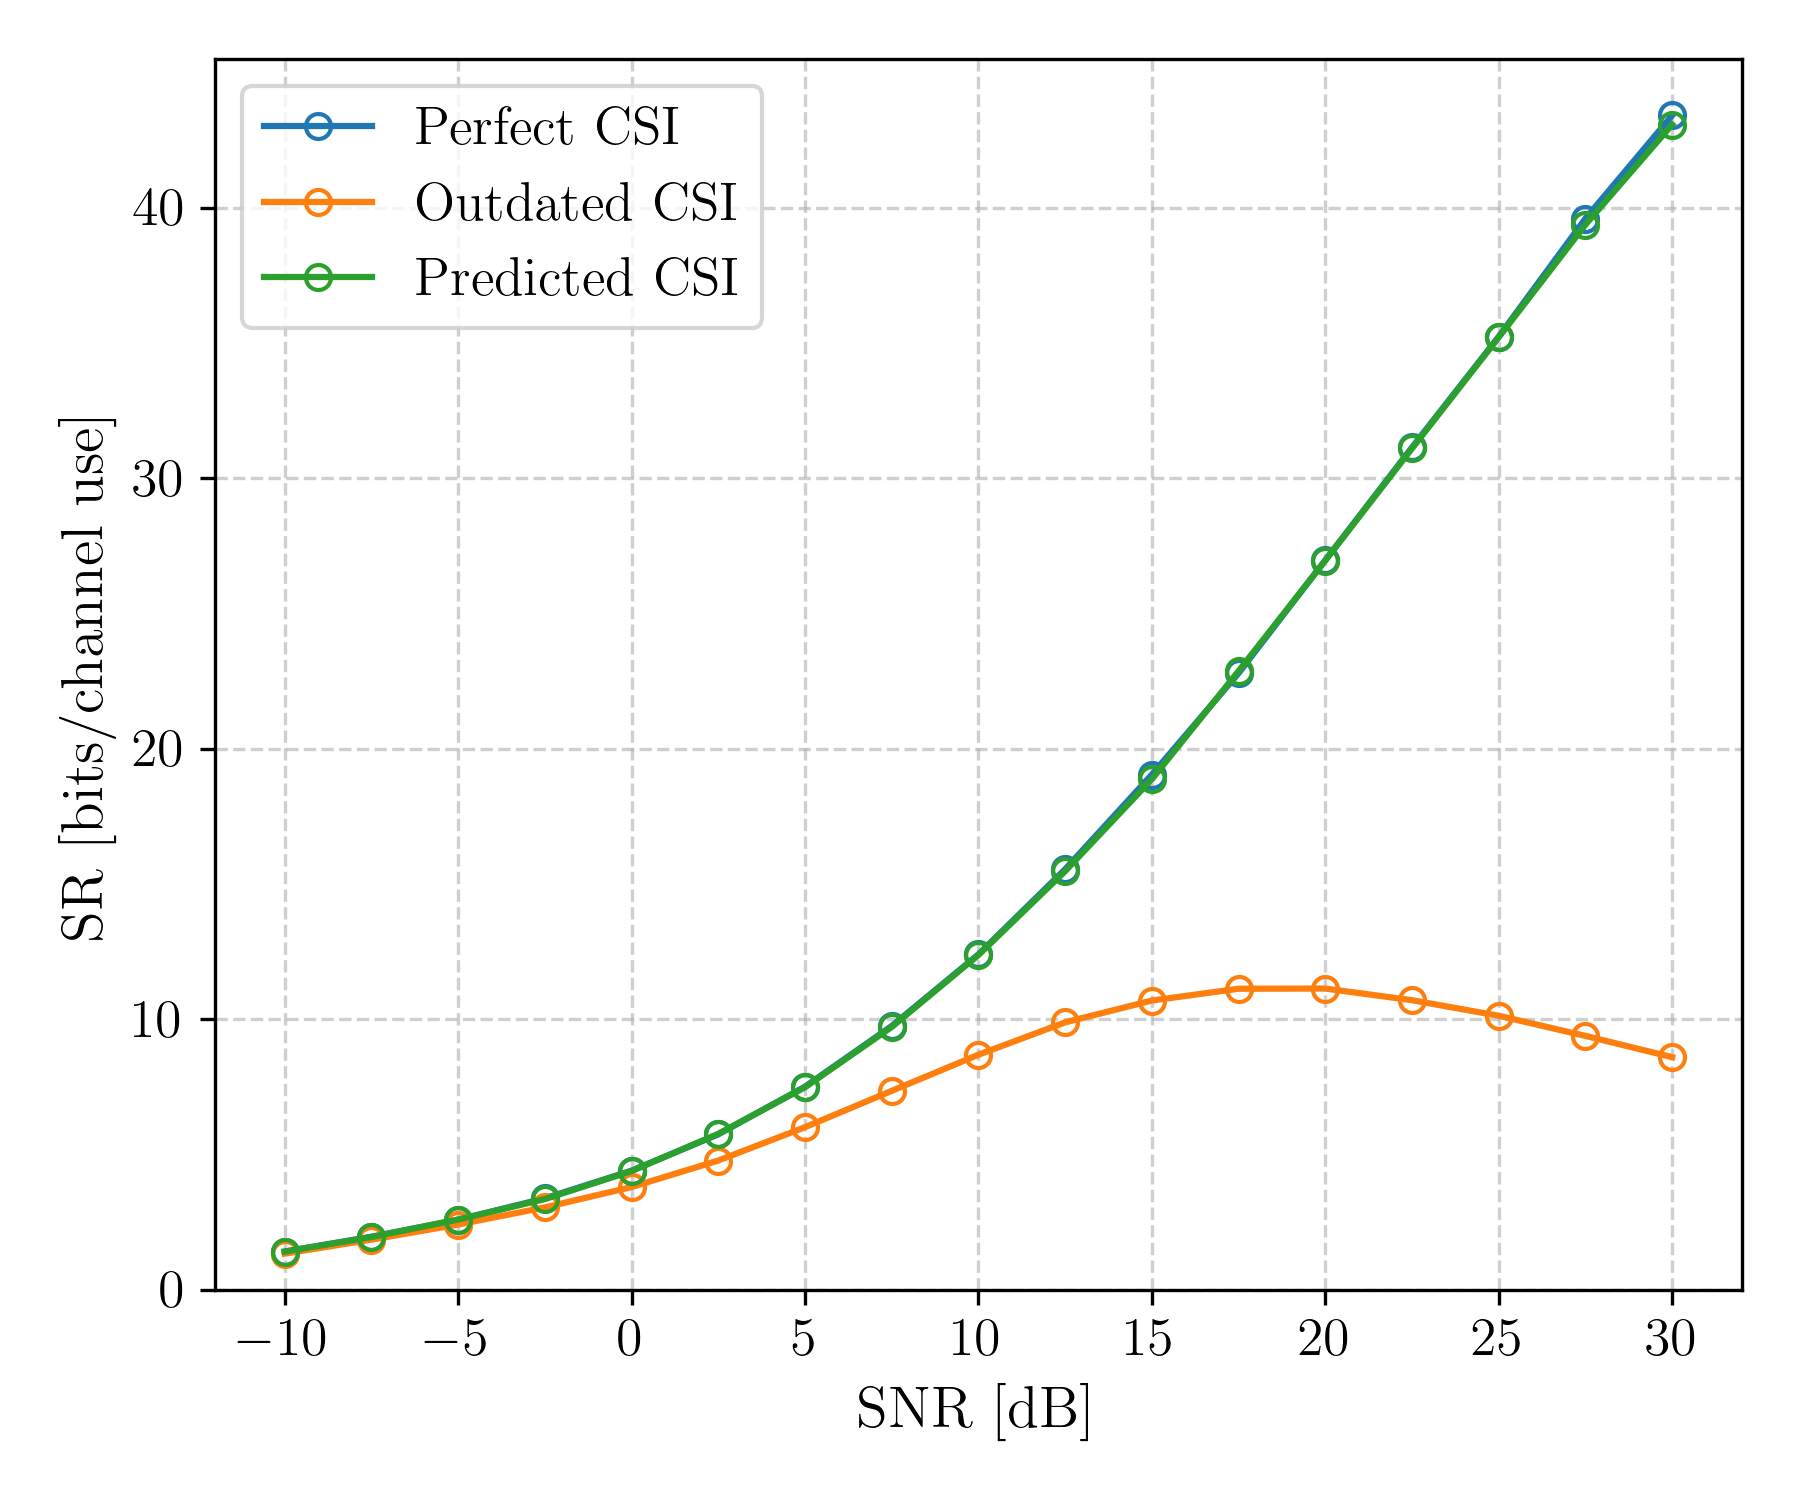
\includegraphics[width=\textwidth]{figures/mobile_satellite_systems/06_precoding_under_outdated_csi/rician_channel/impact_compensation/comparisons/wmmse/2on4.png}
                \caption{$\tau_{\mathrm{CSI}} = \frac{2}{4} T_c$}
            \end{subfigure}
            \hfill
            \begin{subfigure}{0.245\textwidth}
                \centering
                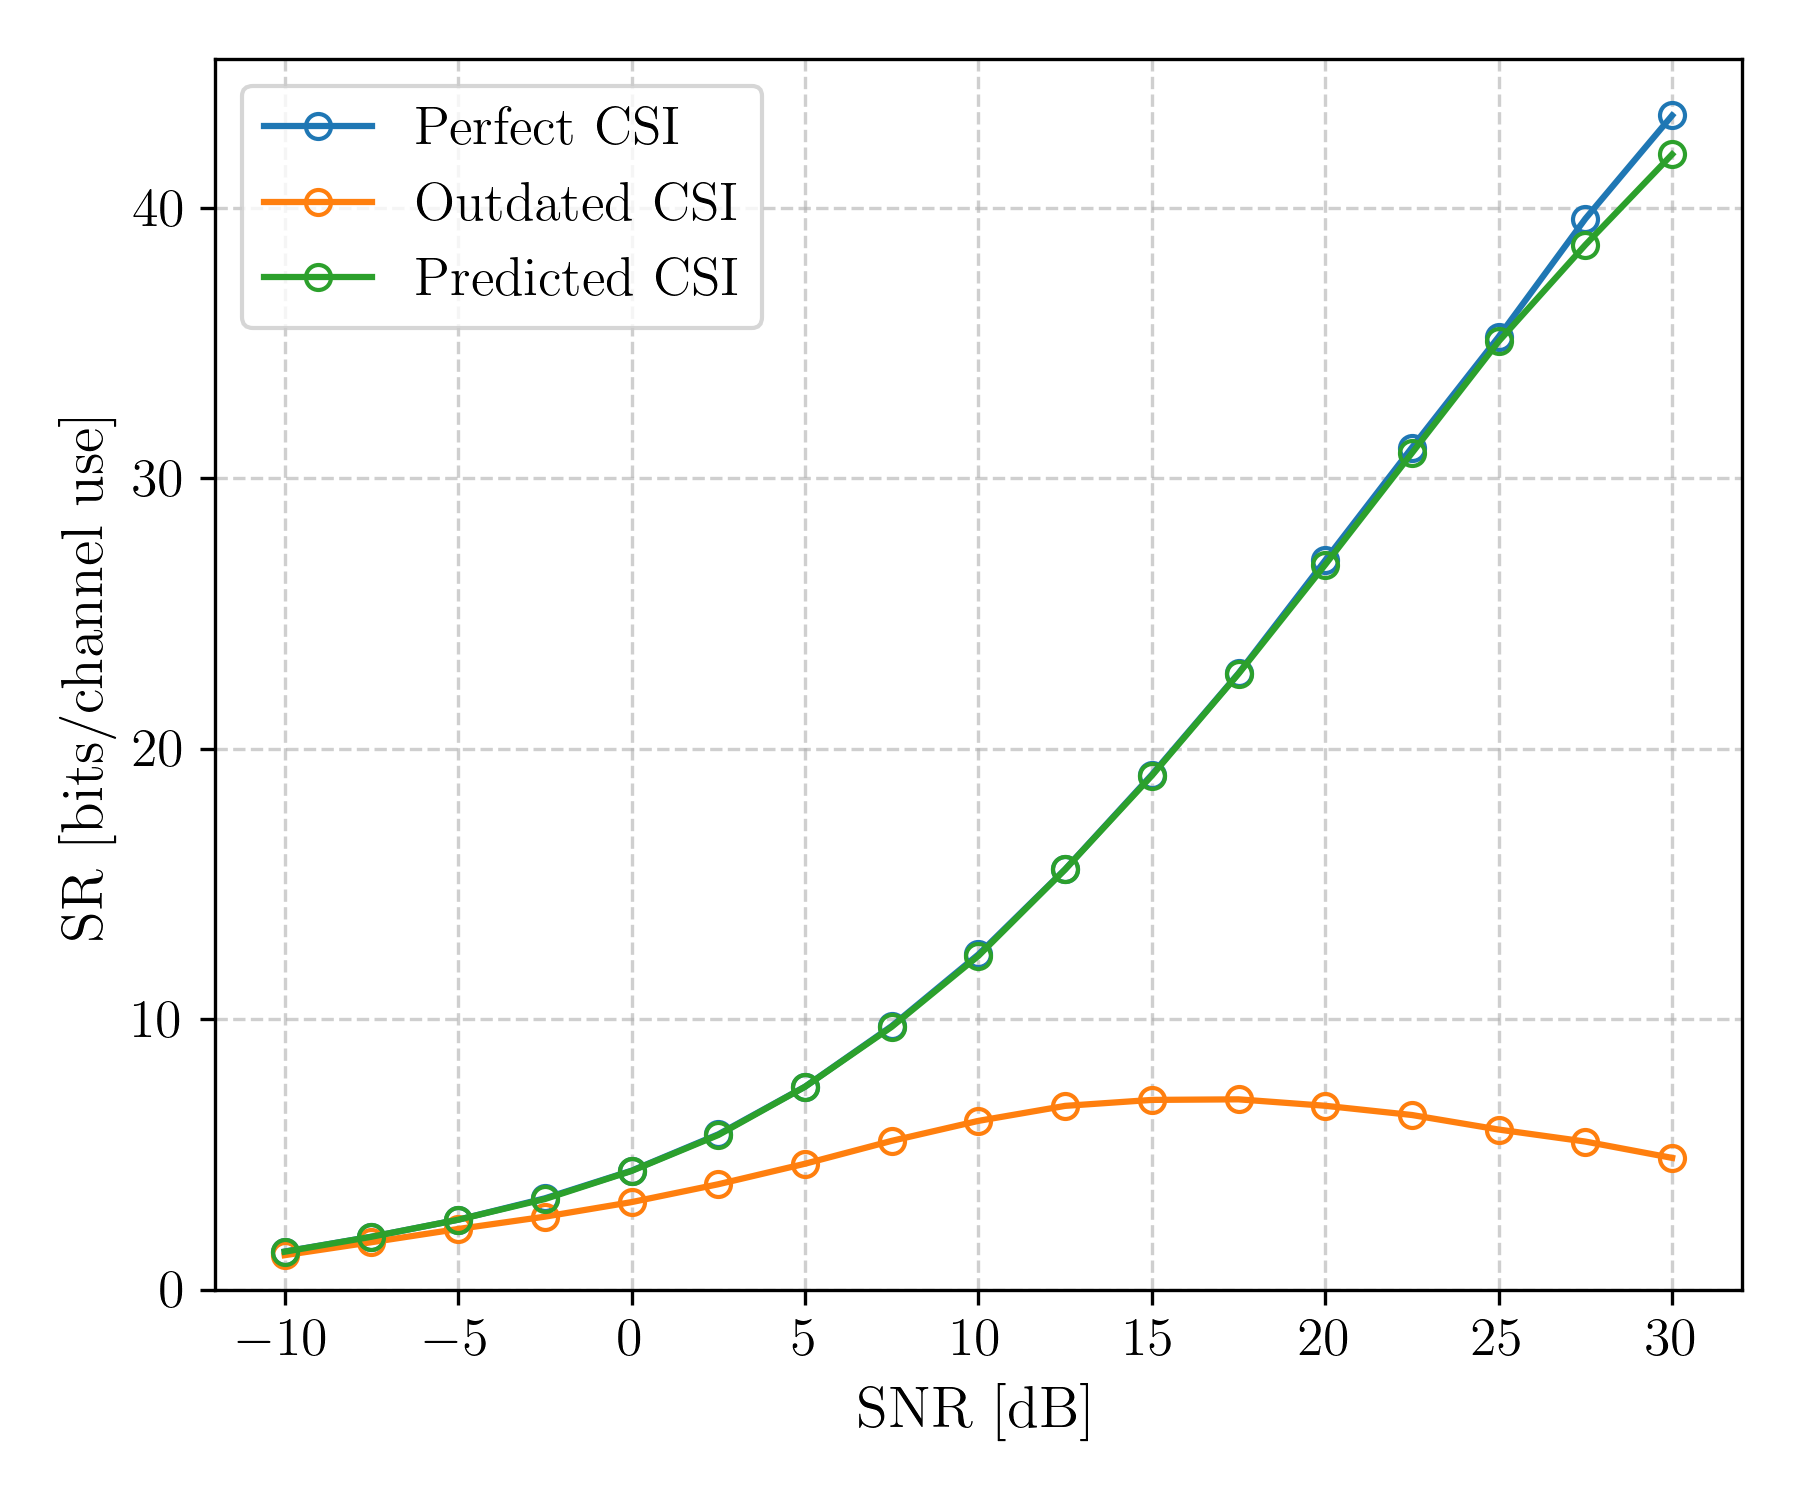
\includegraphics[width=\textwidth]{figures/mobile_satellite_systems/06_precoding_under_outdated_csi/rician_channel/impact_compensation/comparisons/wmmse/3on4.png}
                \caption{$\tau_{\mathrm{CSI}} = \frac{3}{4} T_c$}
            \end{subfigure}
            \hfill
            \begin{subfigure}{0.245\textwidth}
                \centering
                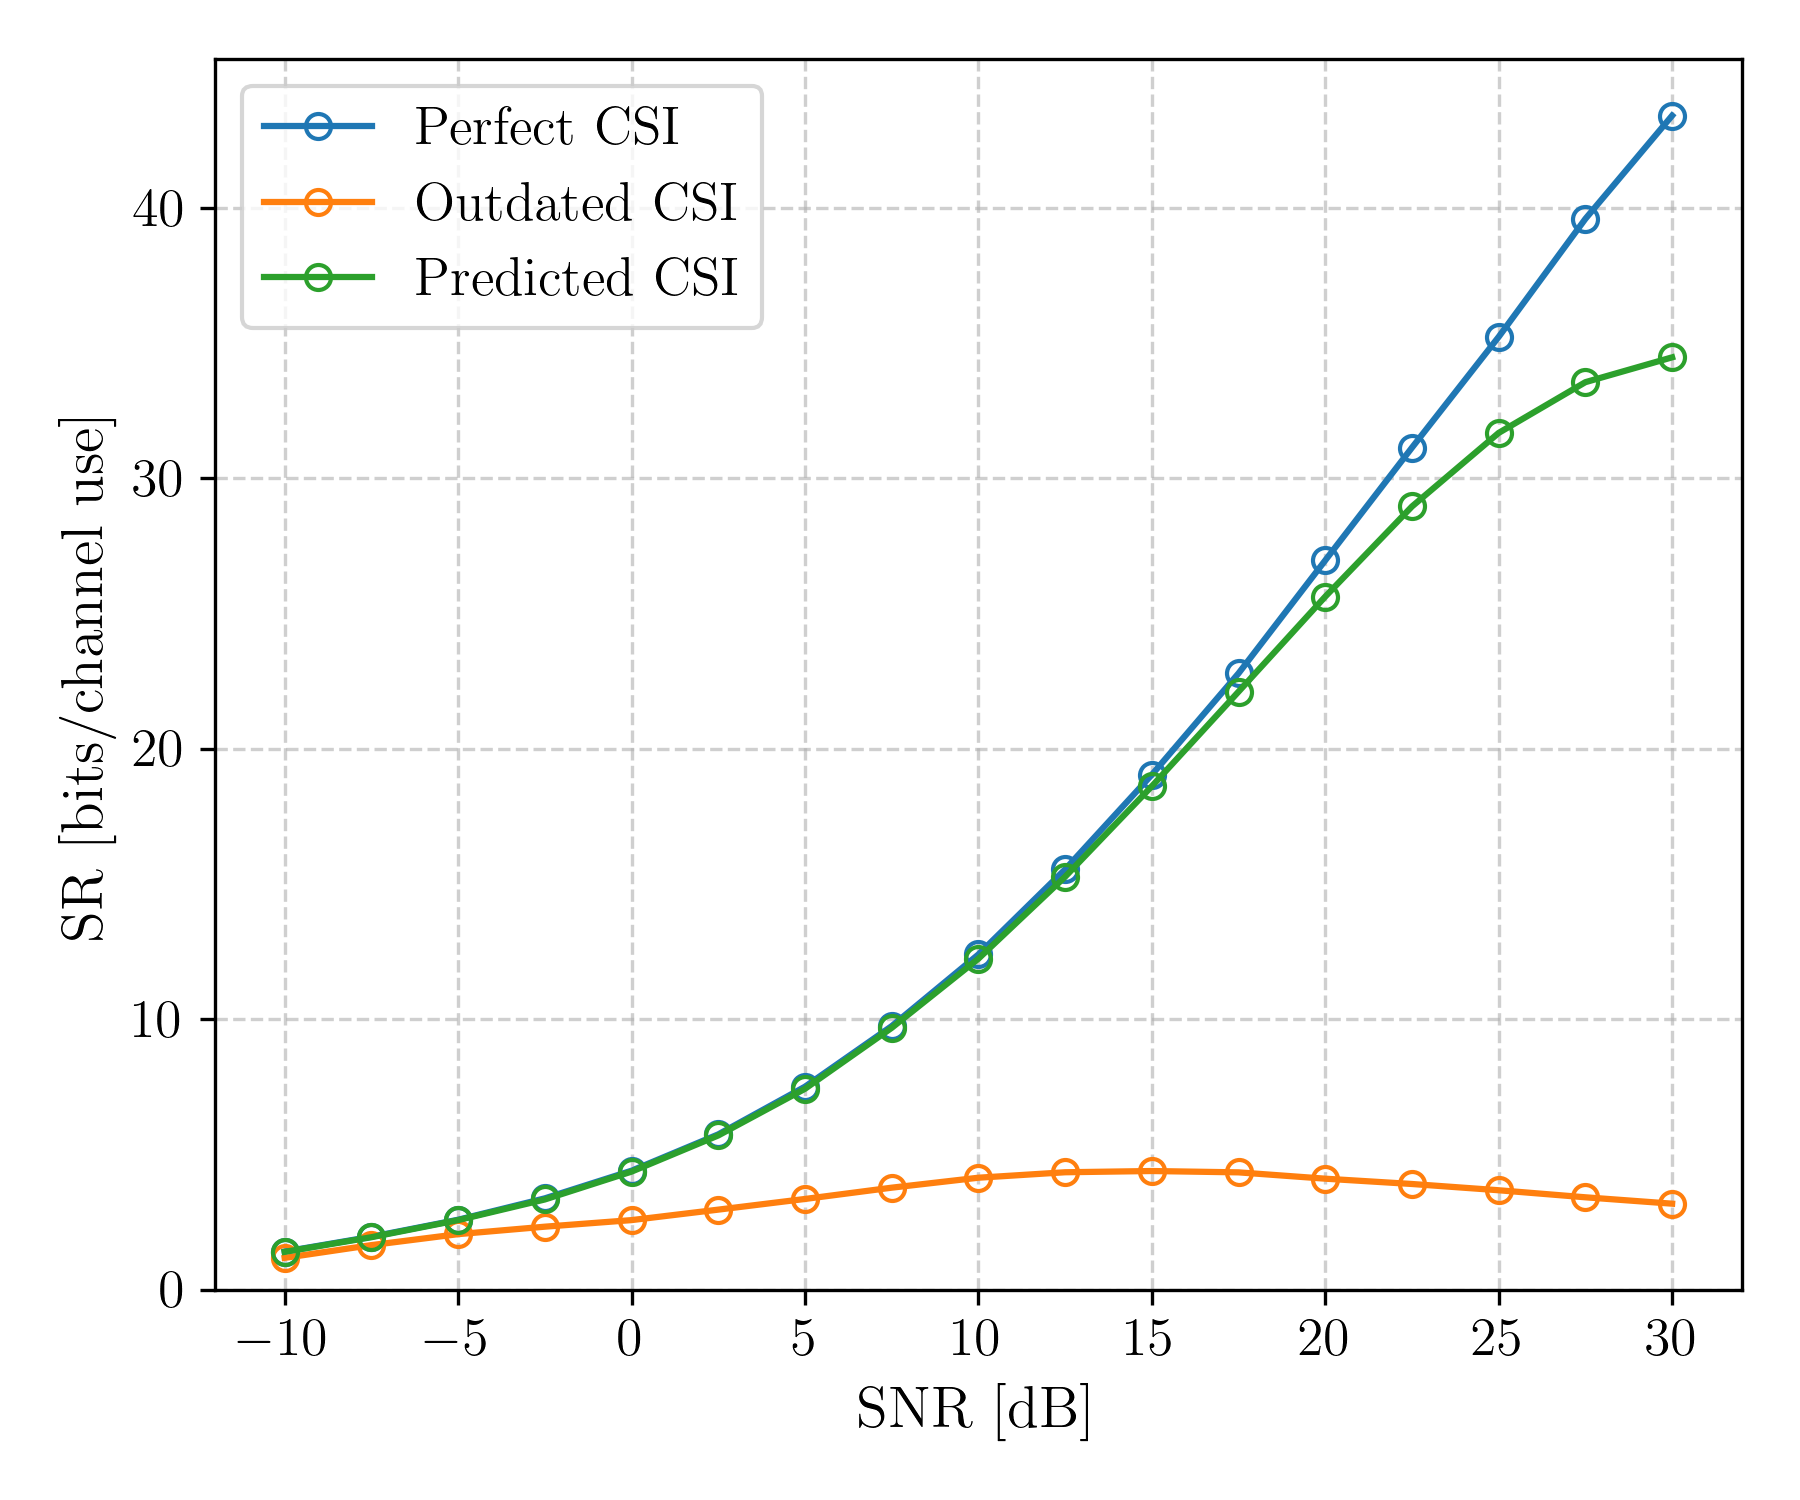
\includegraphics[width=\textwidth]{figures/mobile_satellite_systems/06_precoding_under_outdated_csi/rician_channel/impact_compensation/comparisons/wmmse/4on4.png}
                \caption{$\tau_{\mathrm{CSI}} = \frac{4}{4} T_c$}
            \end{subfigure}

            \vspace{0.5cm}

            % Second row
            \begin{subfigure}{0.245\textwidth}
                \centering
                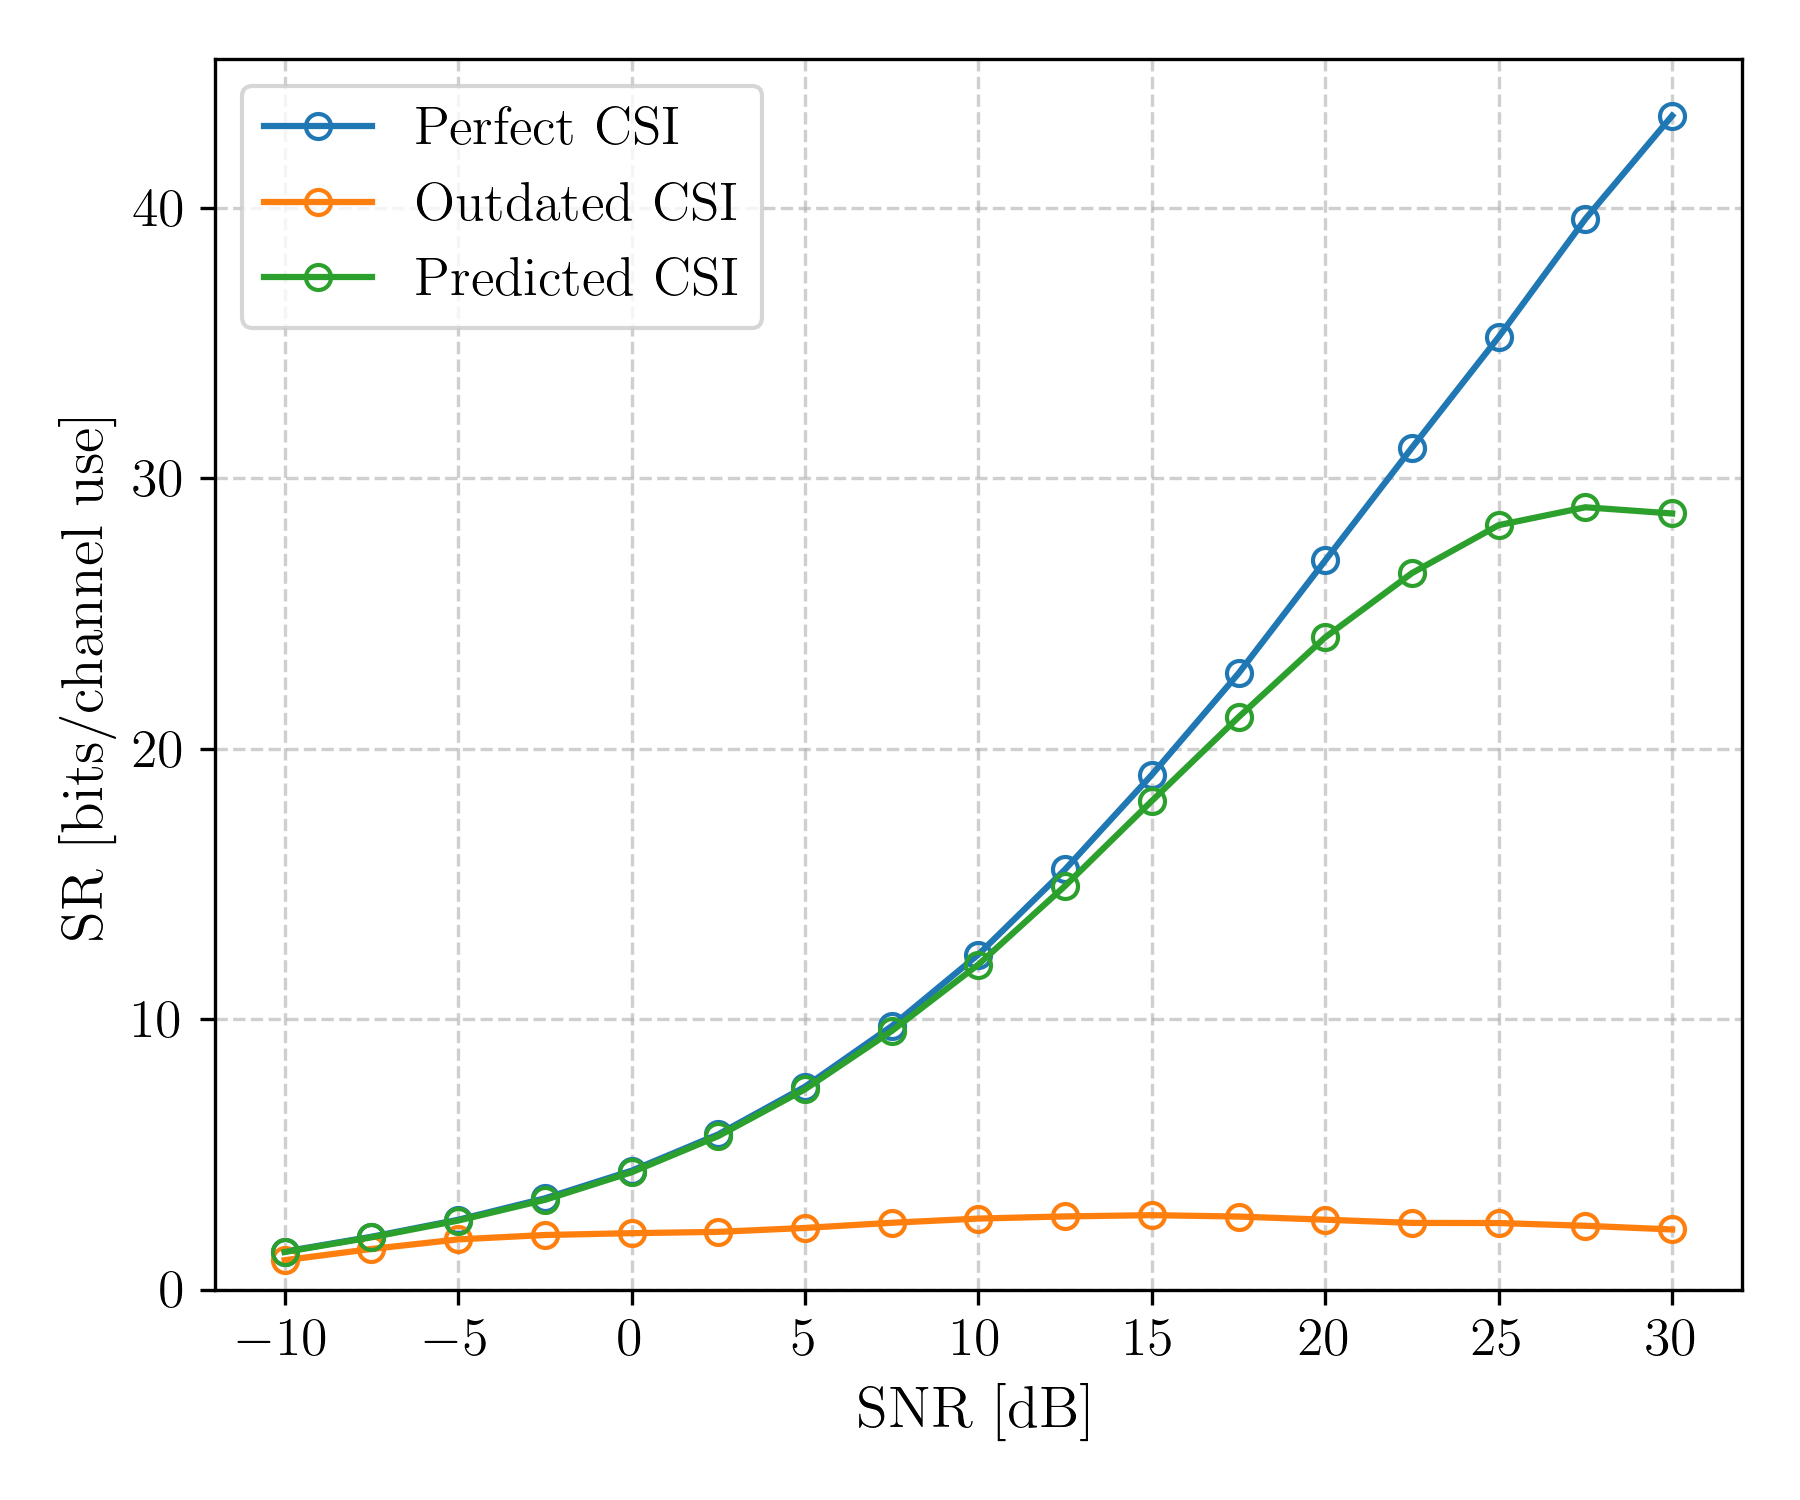
\includegraphics[width=\textwidth]{figures/mobile_satellite_systems/06_precoding_under_outdated_csi/rician_channel/impact_compensation/comparisons/wmmse/5on4.png}
                \caption{$\tau_{\mathrm{CSI}} = \frac{5}{4} T_c$}
            \end{subfigure}
            \hfill
            \begin{subfigure}{0.245\textwidth}
                \centering
                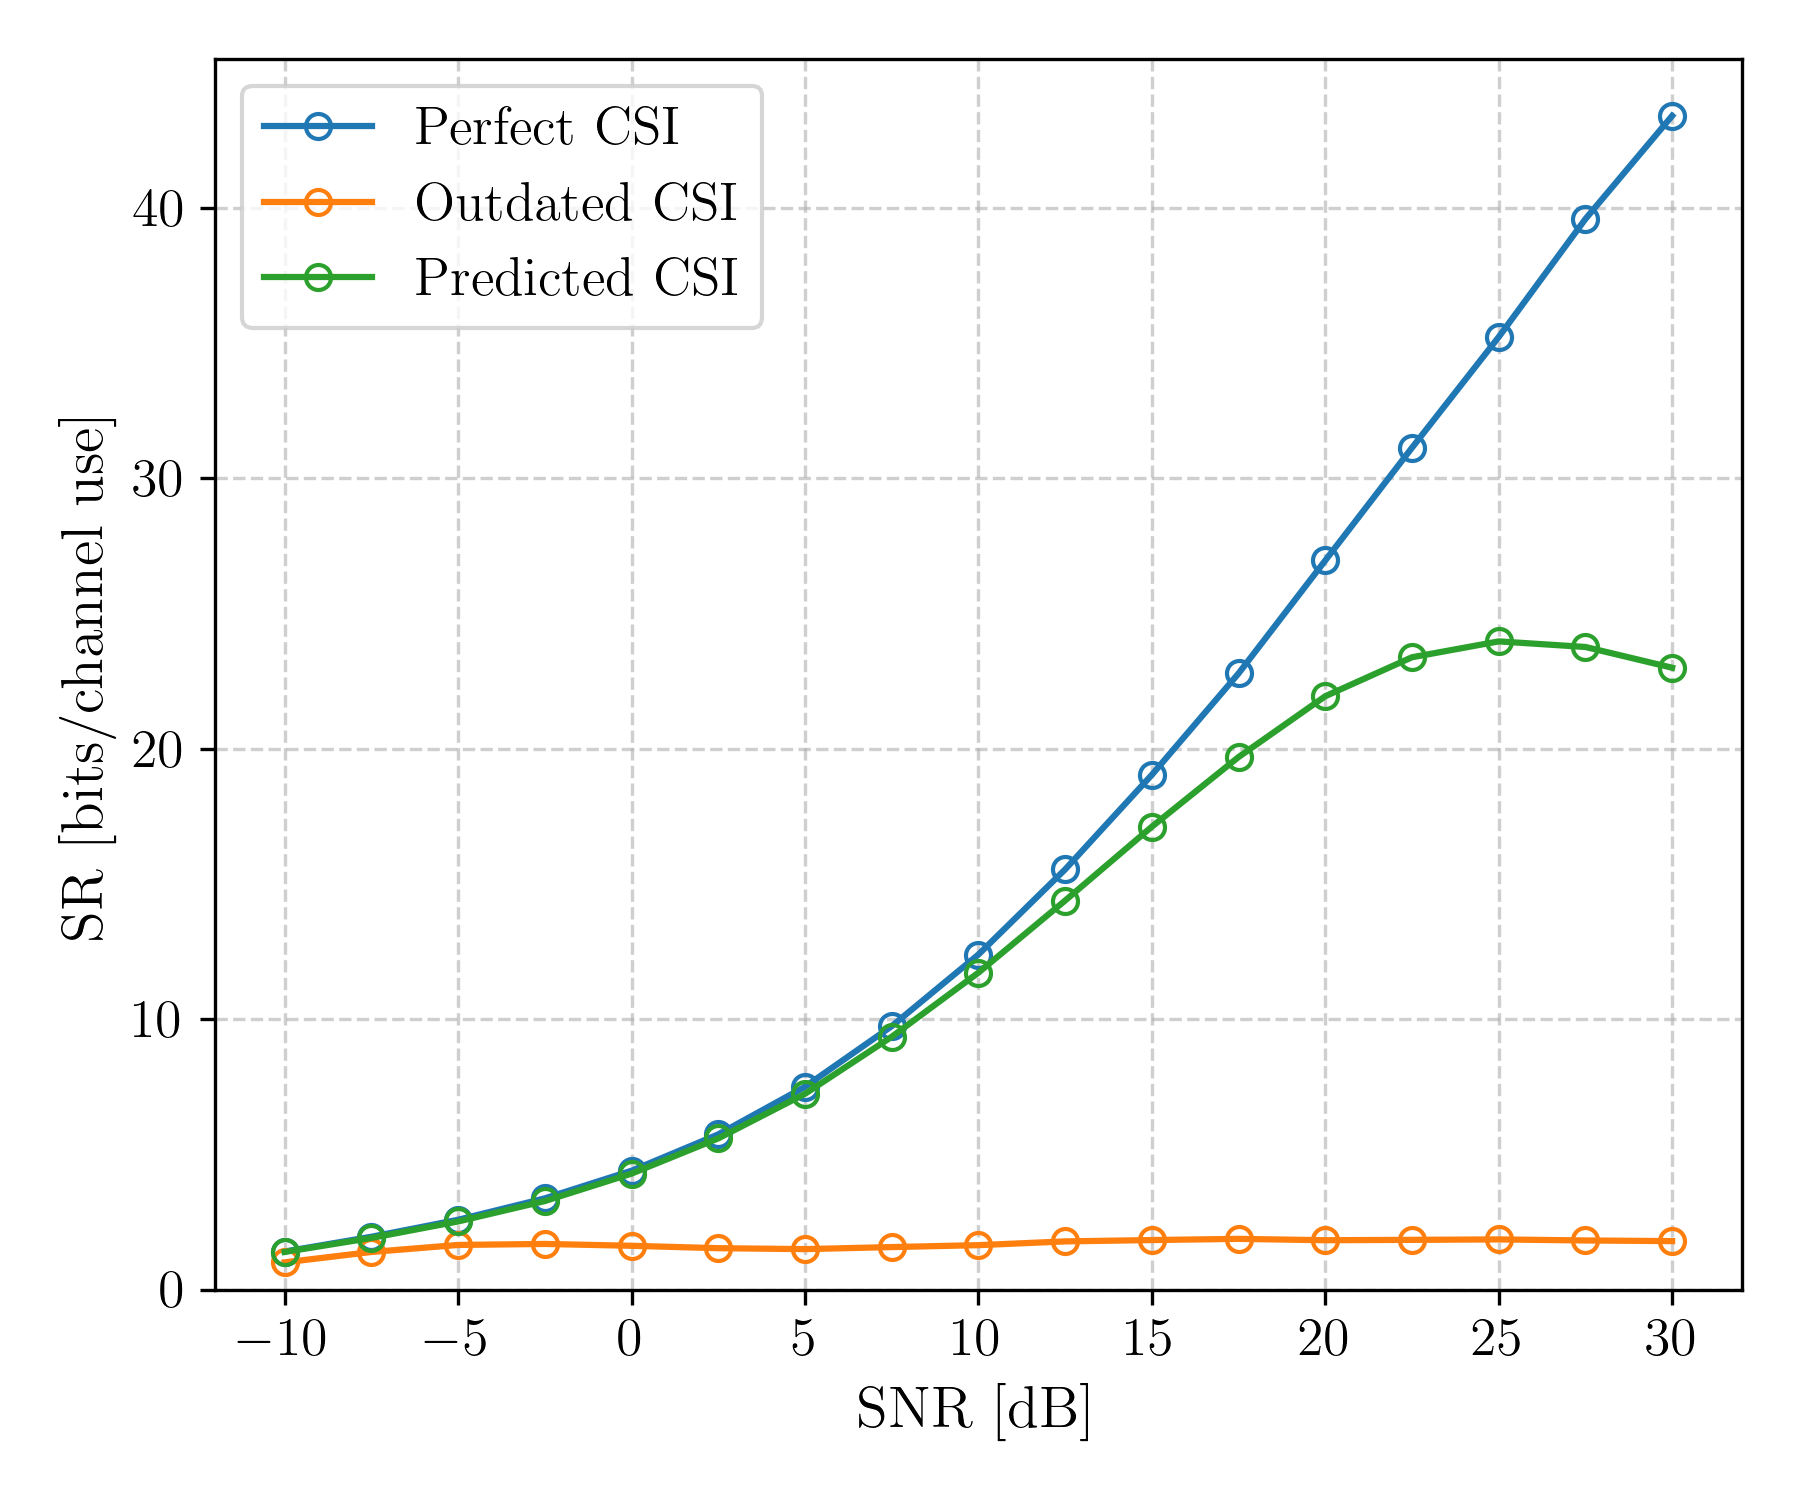
\includegraphics[width=\textwidth]{figures/mobile_satellite_systems/06_precoding_under_outdated_csi/rician_channel/impact_compensation/comparisons/wmmse/6on4.png}
                \caption{$\tau_{\mathrm{CSI}} = \frac{6}{4} T_c$}
            \end{subfigure}
            \hfill
            \begin{subfigure}{0.245\textwidth}
                \centering
                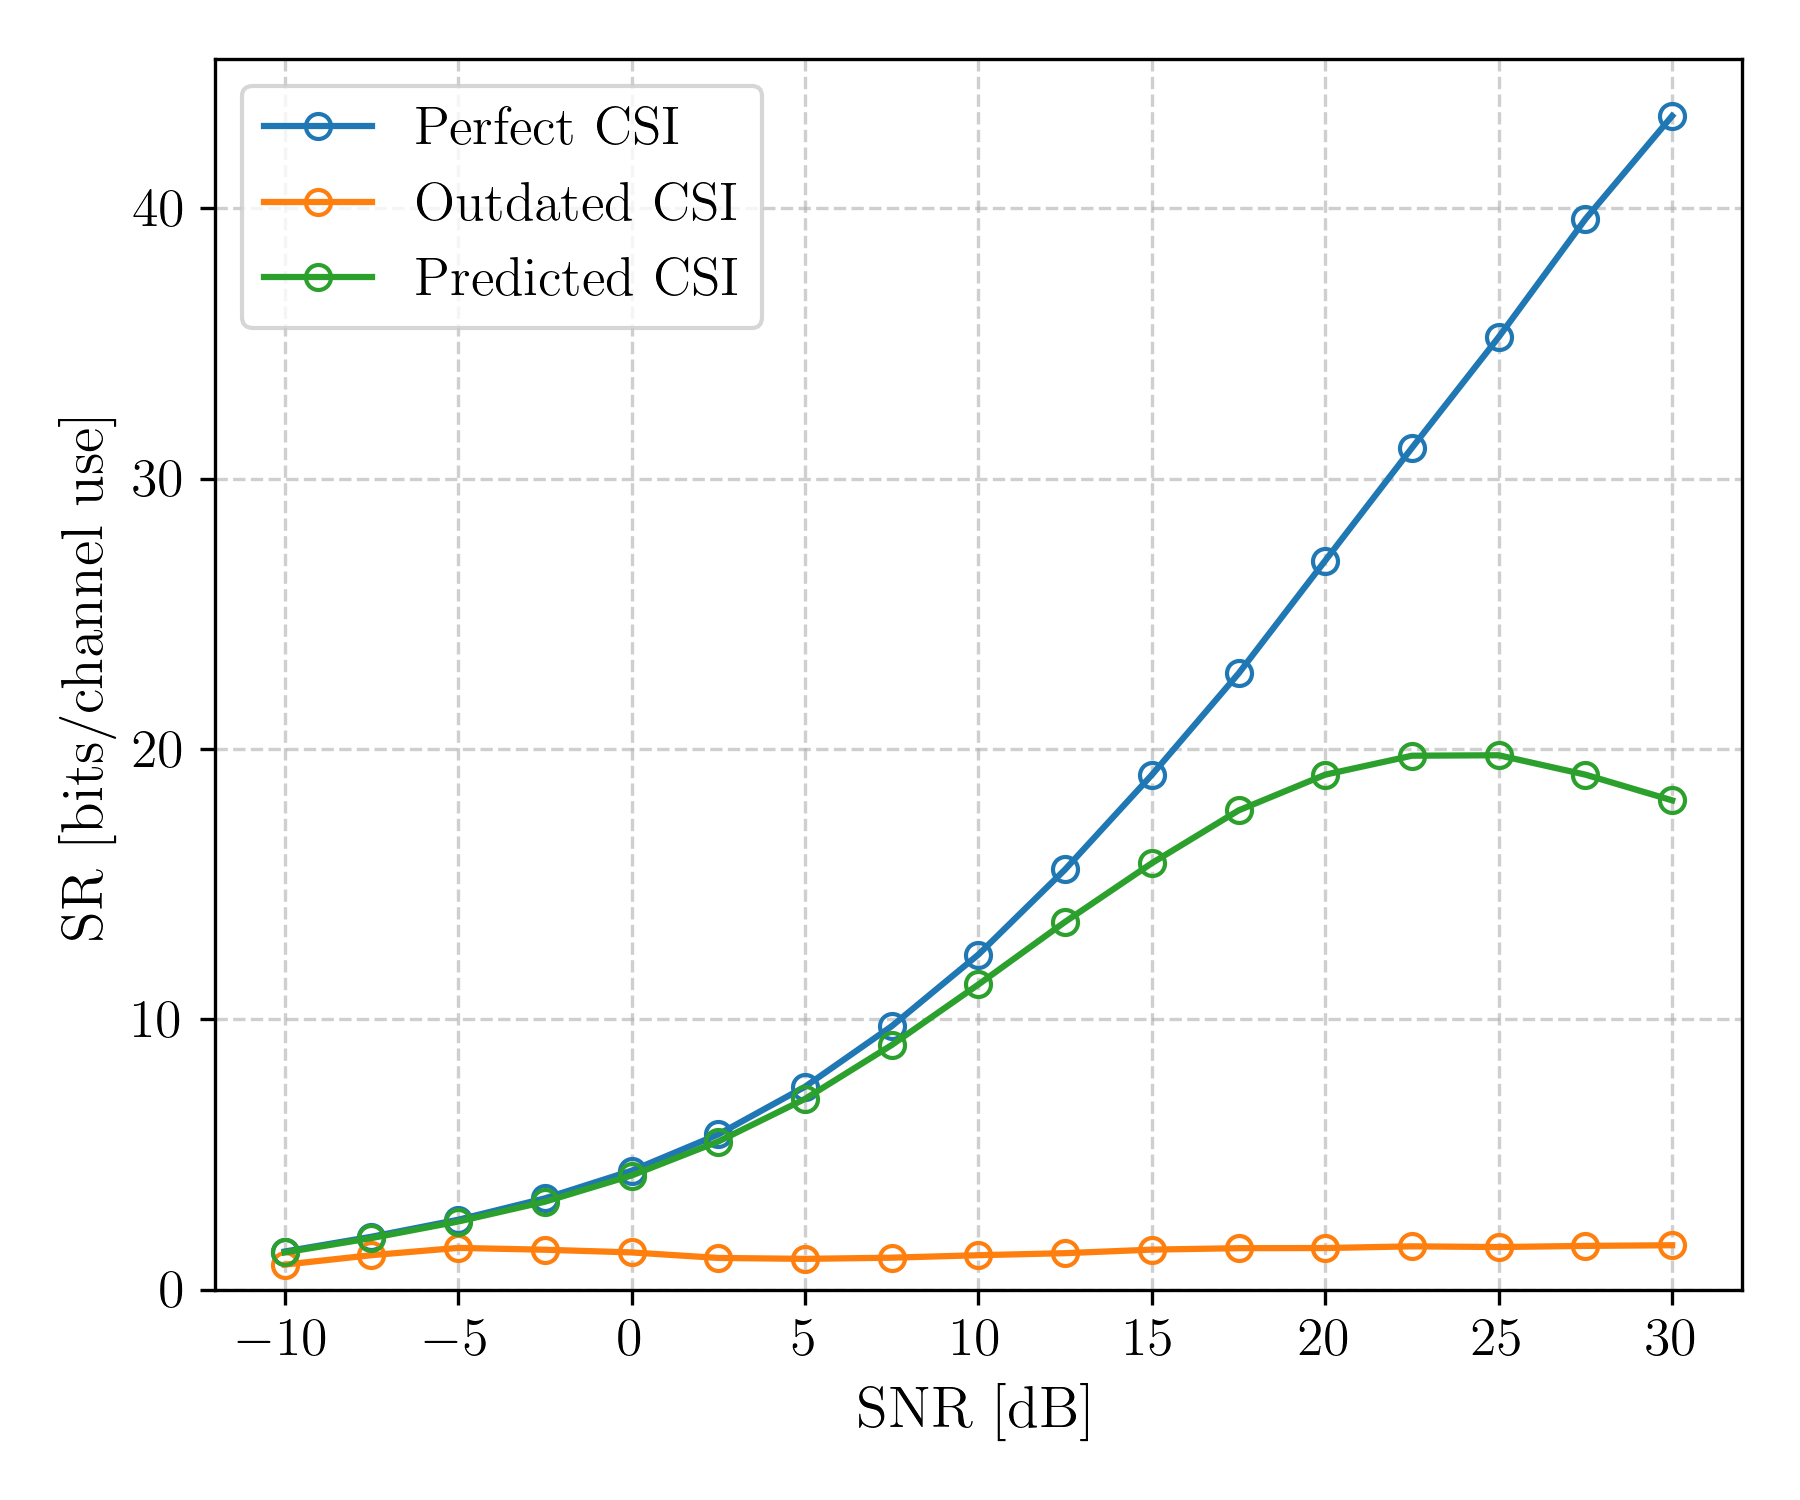
\includegraphics[width=\textwidth]{figures/mobile_satellite_systems/06_precoding_under_outdated_csi/rician_channel/impact_compensation/comparisons/wmmse/7on4.png}
                \caption{$\tau_{\mathrm{CSI}} = \frac{7}{4} T_c$}
            \end{subfigure}
            \hfill
            \begin{subfigure}{0.245\textwidth}
                \centering
                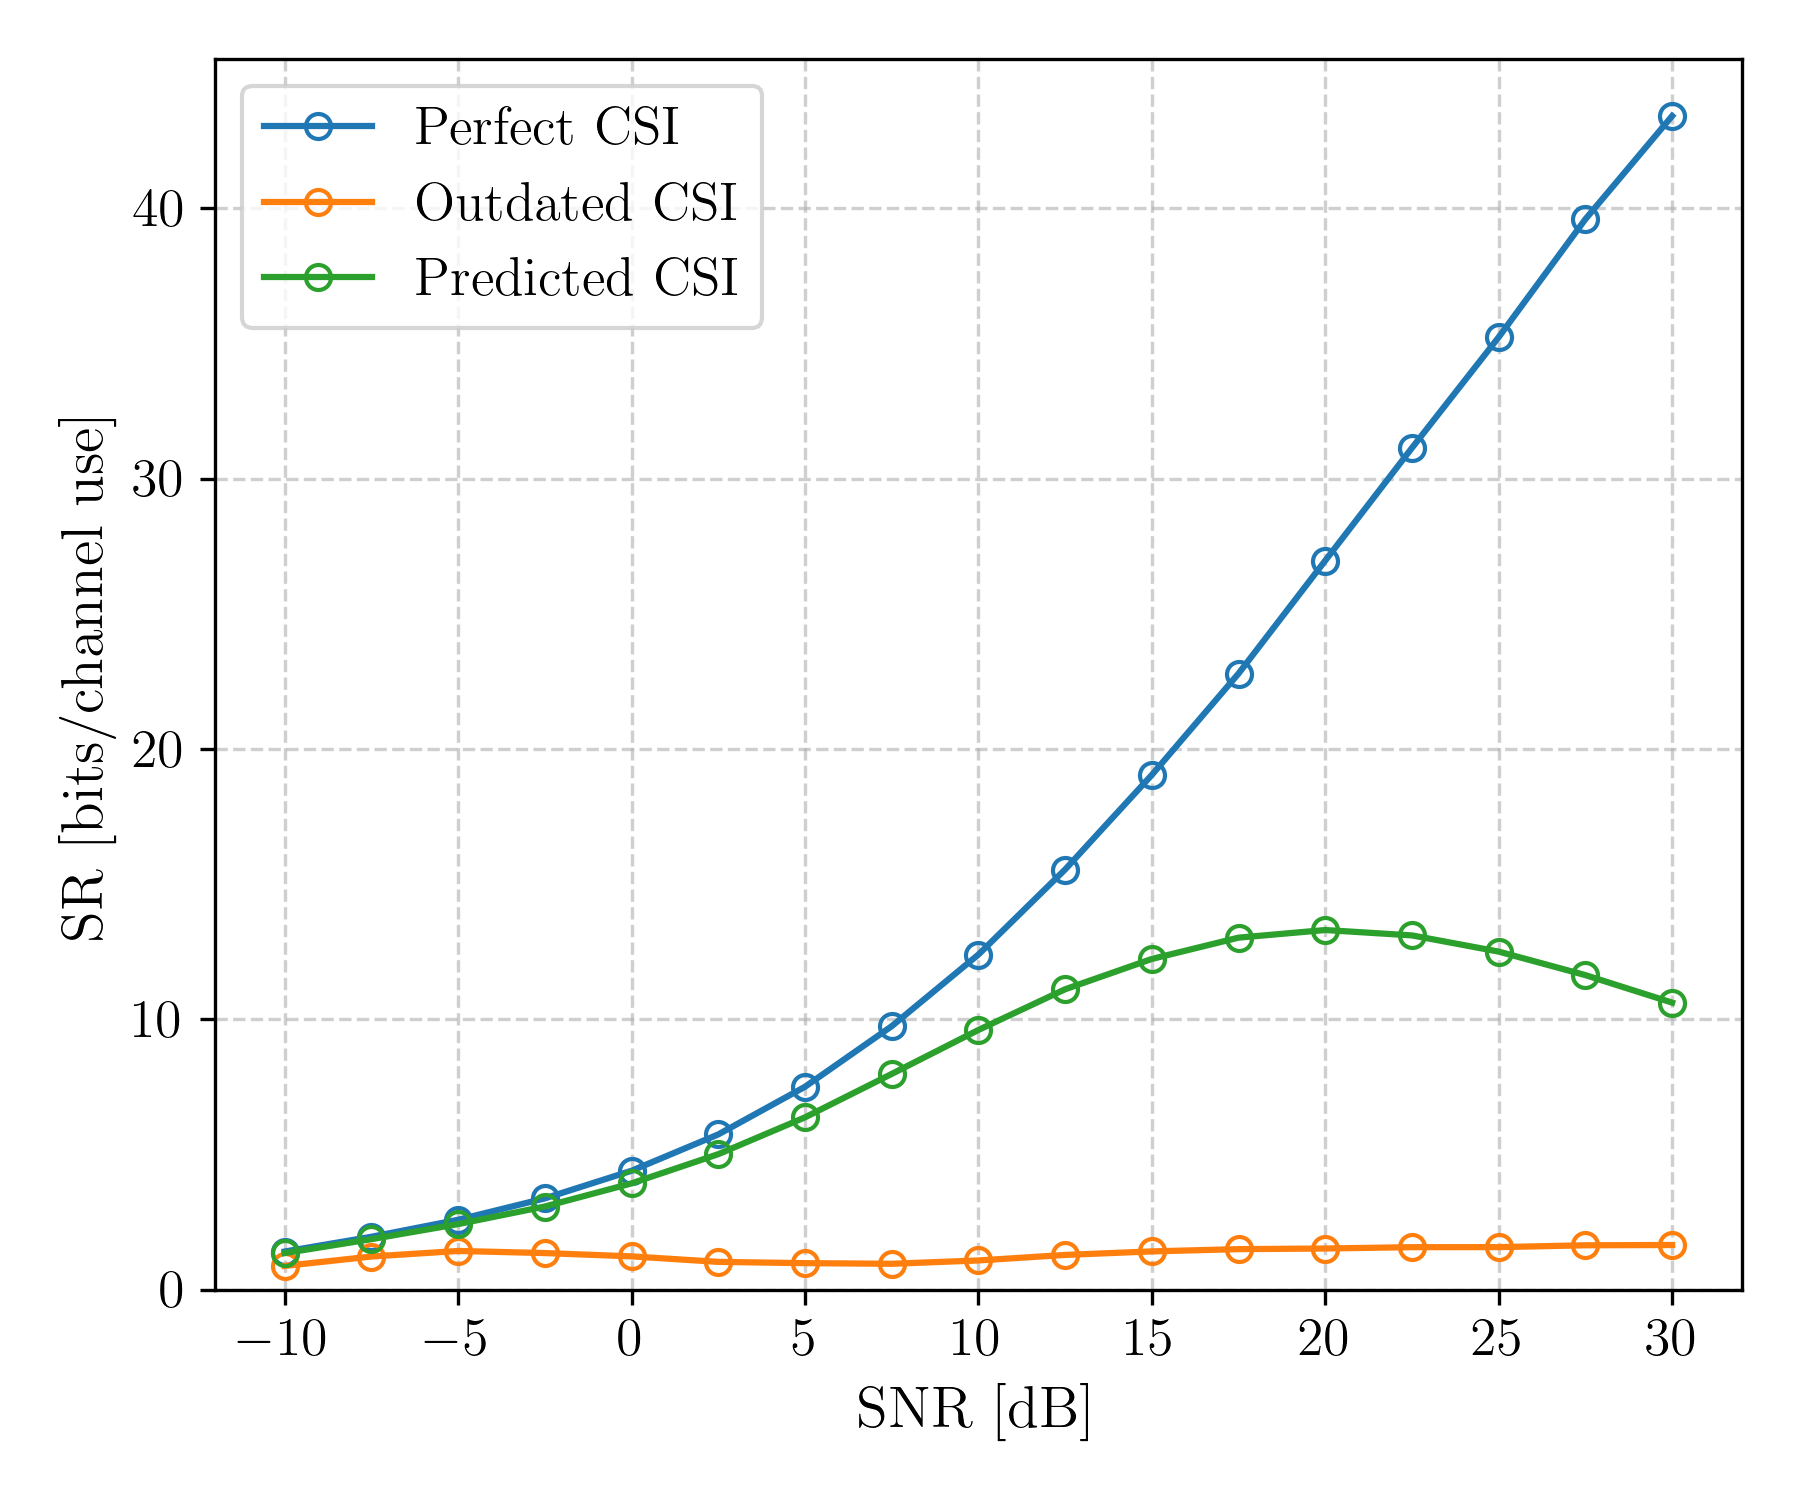
\includegraphics[width=\textwidth]{figures/mobile_satellite_systems/06_precoding_under_outdated_csi/rician_channel/impact_compensation/comparisons/wmmse/8on4.png}
                \caption{$\tau_{\mathrm{CSI}} = \frac{8}{4} T_c$}
            \end{subfigure}

        \end{minipage}
    }

    \caption[Comparison of perfect, outdated and compensated \acs{CSI} for \acs{WMMSE} precoding]{
        A comparison of the \acs{WMMSE} precoding performance under perfect \acs{CSI}, outdated \acs{CSI}, and compensated \acs{CSI} obtained through \acs{AR}-based prediction at the \acp{UT}. 
        The compensation gain is strongest for $\tau_{\mathrm{CSI}} \leq T_c$ and decreases progressively as the feedback delay exceeds the channel coherence time.
    }
    \label{fig:impact_compensation_achievable_rate_wmmse}
\end{figure}

\section{Evaluation on a More Realistic Channel}
\label{section:realistic_channel_evaluation}
% ==============================================
%    Evaluation on a More Realistic Channel
% ==============================================

\subsection{Channel Model}
\label{subsection:realistic_channel_model}

% intro satellite channel
The Rician model used in Sections~\ref{section:outdated_csi_impact} and~\ref{section:outdated_csi_compensation} provides a useful baseline, but it neglects two physically relevant effects in practical mobile satellite links.
First, the antenna array geometry at both the satellite and the \acp{UT} and the propagation directions introduce spatial correlation between channel coefficients.
Second, the motion of a mobile \ac{UT} induces a deterministic Doppler shift on the \ac{LoS} component that cannot always be pre-compensated.
The ray-tracing based channel model introduced in this section extends the Rician model and incorporates both effects. It is based on the channel model from~\cite{8_chinese1_downlink_massive_mimo_leo, chinese0_massive_mimo_leo, 9_chinese2_downlink_robust_precoding}.

% uniform planar array
Both the satellite and each \ac{UT} are equipped with a \acf{UPA}, as illustrated in Figure~\ref{fig:upa}
The satellite array has $N_T = N_T^x \times N_T^y$ elements, with inter-element spacings $d_T^x$ and $d_T^y$ along the x- and y-axis, respectively.
Fully analog, the \ac{UT} array has $N_R = N_R^x \times N_R^y$ elements, with spacings $d_R^x$ and $d_R^y$.
For a wavefront arriving from elevation angle $\theta$ and azimuth angle $\phi$, the array steering vector of a \ac{UPA} with $N = N_x \times N_y$ elements reads
\begin{equation}
\label{eq:upa_steering_vector}
    \mathbf{a}\big(\theta, \phi\big)_{(n_x N_y + n_y)} = \frac{1}{\sqrt{N}} \, \exp\!\left( j\frac{2\pi}{\lambda} \bigl(n_x d_x \sin\theta\cos\phi + n_y d_y \sin\theta\sin\phi\bigr) \right),
\end{equation}
for $n_x = 0, \ldots, N_x - 1$ and $n_y = 0, \ldots, N_y - 1$, where $\lambda$ is the carrier wavelength.

\begin{figure}[!hbt]
    \centering
    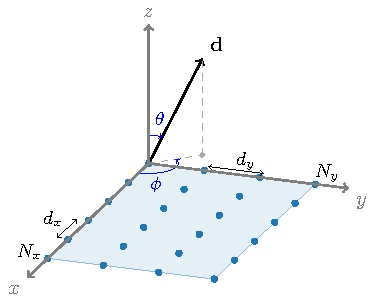
\includegraphics[width=0.5\textwidth]{figures/mobile_satellite_systems/06_precoding_under_outdated_csi/satellite_channel/out/antenna_upa.pdf}
    \caption[Uniform planar array visualization]{
        The uniform planar array (UPA) antenna configuration considered at both the satellite and the \acp{UT}.
        The vector $\mathbf{d}$ points in the satellite-to-user direction.
    }
    \label{fig:upa}
\end{figure}

Because the scattering on ground takes place only within a few kilometers around each \ac{UT}, the \ac{AoD} for different propagation paths to the same \ac{UT} are nearly identical due to the exceptional propagation distance in satellite communications~\cite{chinese0_massive_mimo_leo}.
Therefore, a single satellite-side steering vector $\mathbf{a}^{\mathrm{sat}}_k = \mathbf{a}(\theta^{\mathrm{sat}}_k, \phi^{\mathrm{sat}}_k) \in \mathbb{C}^{N_T}$ applies to every component of the channel, where $(\theta^{\mathrm{sat}}_k, \phi^{\mathrm{sat}}_k)$ is the elevation-azimuth angle pair to \ac{UT}~$k$ from the satellite's point of view.
By contrast, from a \ac{UT} perspective scattering is local, so each ray within a cluster arrives from a distinct direction described by an individual steering vector $\mathbf{a}^{\mathrm{ut}}_{k,c,\ell} = \mathbf{a}(\theta^{\mathrm{ut}}_{k,c,\ell}, \phi^{\mathrm{ut}}_{k,c,\ell}) \in \mathbb{C}^{N_R}$.

% channel matrix 
The channel matrix for \ac{UT}~$k$ is modelled as
\begin{equation}
\label{eq:satellite_channel_model}
\begin{aligned}
    &\mathbf{H}_k(t) = \sqrt{\frac{\kappa}{\kappa+1}} \; \mathbf{H}_k^{\mathrm{LoS}}(t) + \sqrt{\frac{1}{\kappa+1}} \; \mathbf{H}_k^{\mathrm{NLoS}}(t) \\
    &\text{with} \quad \mathbf{H}_k^{\mathrm{LoS}}(t) = \alpha_k^{\mathrm{LoS}}(t) \; \mathbf{a}^{\mathrm{ut}}_k \bigl(\mathbf{a}^{\mathrm{sat}}_k\bigr)^{\!\mathsf{H}} \\
    &\text{and } \quad \mathbf{H}_k^{\mathrm{NLoS}}(t) = \sum_{c=1}^{C} \sqrt{w_c} \cdot \frac{1}{\sqrt{L_c}} \sum_{\ell=1}^{L_c} \alpha_{k,c,\ell}^{\mathrm{NLoS}}(t) \; \mathbf{a}^{\mathrm{ut}}_{k,c,\ell} \bigl(\mathbf{a}^{\mathrm{sat}}_k\bigr)^{\!\mathsf{H}},
\end{aligned}
\end{equation}
where $\kappa$ is the Rician factor, $c$ indexes the \ac{NLoS} scattering clusters with relative powers $w_c$, and $L_c$ is the number of rays
in cluster $c$.

% LoS component
The \ac{LoS} gain $\alpha_k^{\mathrm{LoS}}(t)$ incorporates the Doppler shift induced by the \ac{UT}'s motion:
\begin{equation}
\label{eq:los_gain}
    \alpha_k^{\mathrm{LoS}}(t) = \exp\bigl(j\bigl(\psi_k + 2\pi\nu_k^{\mathrm{LoS}}\,t\bigr)\bigr),
\end{equation}
where $\psi_k \sim \mathcal{U}(0, 2\pi)$ is a random initial phase and $\nu_k^{\mathrm{LoS}} = f_D \, \cos(\pi/2 - \theta^{\mathrm{sat}}_k)$ is the Doppler frequency of the \ac{LoS} path.
Here, $f_D = v_{\mathrm{UT}} \, f_c / c$ is the maximum Doppler frequency, determined by the carrier frequency $f_c$, the \ac{UT} velocity $v_{\mathrm{UT}}$, and the speed of light $c$.
The factor $\sin\theta^{\mathrm{sat}}_k$ accounts for the projection of the \ac{UT}'s horizontal velocity onto the satellite-to-user direction.
Unlike the simplified model of~\eqref{eq:rician_channel_model}, the \ac{LoS} component is no longer time-invariant. It rotates in phase at a rate that depends on the \ac{UT}'s velocity and elevation angle.

% NLoS component
Each cluster consists of $L_c$ rays whose temporal evolution follows the same Jakes isotropic-scattering model as in the simplified channel of
Section~\ref{section:outdated_csi_problem_formulation}.
\begin{equation}
\label{eq:nlos_gain}
    \alpha_k^{\mathrm{NLoS}}(t) \sim \mathcal{CN}(0, 1) \quad \text{with} \quad R_{\alpha_k^{\mathrm{NLoS}}}(\Delta t) = J_0(2\pi f_D \Delta t).
\end{equation}
The \ac{AoA} at \ac{UT}~$k$ of a ray $\ell$ within cluster $c$ is
\begin{align}
    \theta^{\mathrm{ut}}_{k,c,\ell} &= \theta^{\mathrm{ut}}_k + \Delta\theta_{k,c} + \sigma_\theta\, u_{k,c,\ell},
    \label{eq:nlos_elevation_angles}\\
    \phi^{\mathrm{ut}}_{k,c,\ell} &= \phi^{\mathrm{ut}}_k + \Delta\phi_{k,c} + \sigma_\phi\, v_{k,c,\ell},
    \label{eq:nlos_azimuth_angles}
\end{align}
where $(\theta^{\mathrm{ut}}_k, \phi^{\mathrm{ut}}_k)$ is the \ac{LoS} direction as seen at the \ac{UT}, $(\Delta\theta_{k,c}, \Delta\phi_{k,c})$ is the mean angular offset from the \ac{LoS} direction for cluster $c$, $\sigma_\theta$ and $\sigma_\phi$ are the intra-cluster angular spreads, and $u_{k,c,\ell}$, $v_{k,c,\ell}$ are independent Laplace-distributed random variables with zero mean and unit variance.
We restrict ourselves to $2$ clusters.
The first cluster is centred on the \ac{LoS} direction ($\Delta\theta_{k,1} = \Delta\phi_{k,1} = 0$), while the second cluster is offset by a user-specific, randomly drawn displacement $(\Delta\theta_{k,2}, \Delta\phi_{k,2})$.
The elevation angle of the \ac{LoS} path is the same at both the satellite and the \ac{UT}, i.e. $\theta^{\mathrm{ut}}_k = \theta^{\mathrm{sat}}_k$.
The orientation of the \ac{UT}'s array, i.e. $\phi^{\mathrm{ut}}_k$, relative to the satellite's array is determined by a rotation $\rho$ around the vertical axis, which is uniformly distributed in $[0, 2\pi)$ and independent of the satellite-side azimuth.
\medskip

% important distinct characteristics.
Since every term in~\eqref{eq:satellite_channel_model} shares the same satellite-side steering vector $\mathbf{a}^{\mathrm{sat}}_k$, the channel matrix of a single \ac{UT} is of rank one at any moment in time.
Consequently, regardless of the number of receive antennas, the channel of each \ac{UT} supports at most one spatial stream.
This significantly alters the behavior of the precoding schemes considered in this work, since the receive-side spatial multiplexing gain is no longer available.
Because the purpose of this section is not to study this rank limitation itself, the subsequent evaluation is restricted to system configurations in which each \ac{UT} is equipped with a single receive antenna.

A second distinction from the simplified model concerns the spatial structure of the channel.
Under the ray-based model of~\eqref{eq:satellite_channel_model}, the entries of the channel matrix for \ac{UT}~$k$ are no longer spatially independent.
In principle, a predictor that exploits this spatial correlation jointly with the temporal one could yield more accurate predictions than the element-wise approach of Section~\ref{subsection:compensation_strategy}.
However, developing such a predictor would significantly increase the complexity at each \ac{UT}.
To maintain a fair and direct comparison with the results of Section~\ref{section:outdated_csi_compensation}, the same element-wise \ac{AR} predictor is applied here without modification, with the same parameter values established in Section~\ref{subsection:compensation_parameter_optimization}.

\subsection{Performance Evaluation}
\label{subsection:performance_evaluation}
% ----------------------------------------

% intro / setup
In this section, we perform a first evaluation of the \ac{BER} of an $8 \times \{1,1,1,1\}$ system using a \ac{ZF} precoder. Each \ac{UT} is equipped with a single receive antenna and is served with one data stream carrying $16$-\ac{QAM} symbols.
In analogy with Section~\ref{section:outdated_csi_impact}, the \ac{CSI} feedback delay is expressed as a fraction of the coherence time $T_c$ of the \ac{NLoS} component, as defined in~\eqref{eq:coherence_time_def}, so that the results remain independent of any particular choice of \ac{UT} velocity or carrier frequency.

% outdated CSI
The left panel of Figure~\ref{fig:satellite_channel_performance} shows the \ac{BER} under outdated \ac{CSI} as a function of the \ac{SNR} for several values of the feedback delay.
The qualitative behavior closely mirrors the observations made in Section~\ref{section:outdated_csi_impact} for the simplified Rician model.
As the feedback delay grows, the \ac{BER} at any given \ac{SNR} degrades monotonically.
For delays approaching or exceeding $T_c^{\mathrm{NLoS}}$, the residual inter-user interference caused by the channel mismatch begins to dominate the noise at high \ac{SNR}, and the \ac{BER} curves flatten. The system has an extremely poor reliability, no matter the available transmit power.

% compensation
The right panel of Figure~\ref{fig:satellite_channel_performance} shows the same system with \ac{AR}-based channel prediction.
The compensation restores a substantial fraction of the performance lost due to the feedback delay, in line with the findings of Section~\ref{subsection:compensation_performance_evaluation}.
A notable difference with respect to the simplified model, however, is that the predictor remains effective over a wider range of \ac{CSI} feedback delays.
This extended compensation range can be attributed to the deterministic \ac{LoS} component.
Because the \ac{LoS} phase rotates at a fixed rate $\nu_k^{\mathrm{LoS}}$ that is fully determined by the satellite geometry and the \ac{UT} velocity, the \ac{AR} model can track this contribution accurately even when the coherence time of the \ac{NLoS} component has been exceeded.

% conclusion
These first results are promising: the \ac{AR}-based compensation strategy, developed and tuned under the simplified Rician model, is capable of significantly reducing the \ac{BER} for feedback delays up to $4$ times the \ac{NLoS} coherence time.
At the same time, these simulations only scratch the surface of what a dedicated analysis of this channel model could reveal.
A thorough parameter study, an investigation of the spatial and temporal correlation structure on precoding performance, and a comparison across multiple precoding strategies are needed to draw sound conclusions, and are left as natural directions for future work.

\begin{figure}[!htb]
    \centering
    \begin{subfigure}{0.495\textwidth}
        \centering
        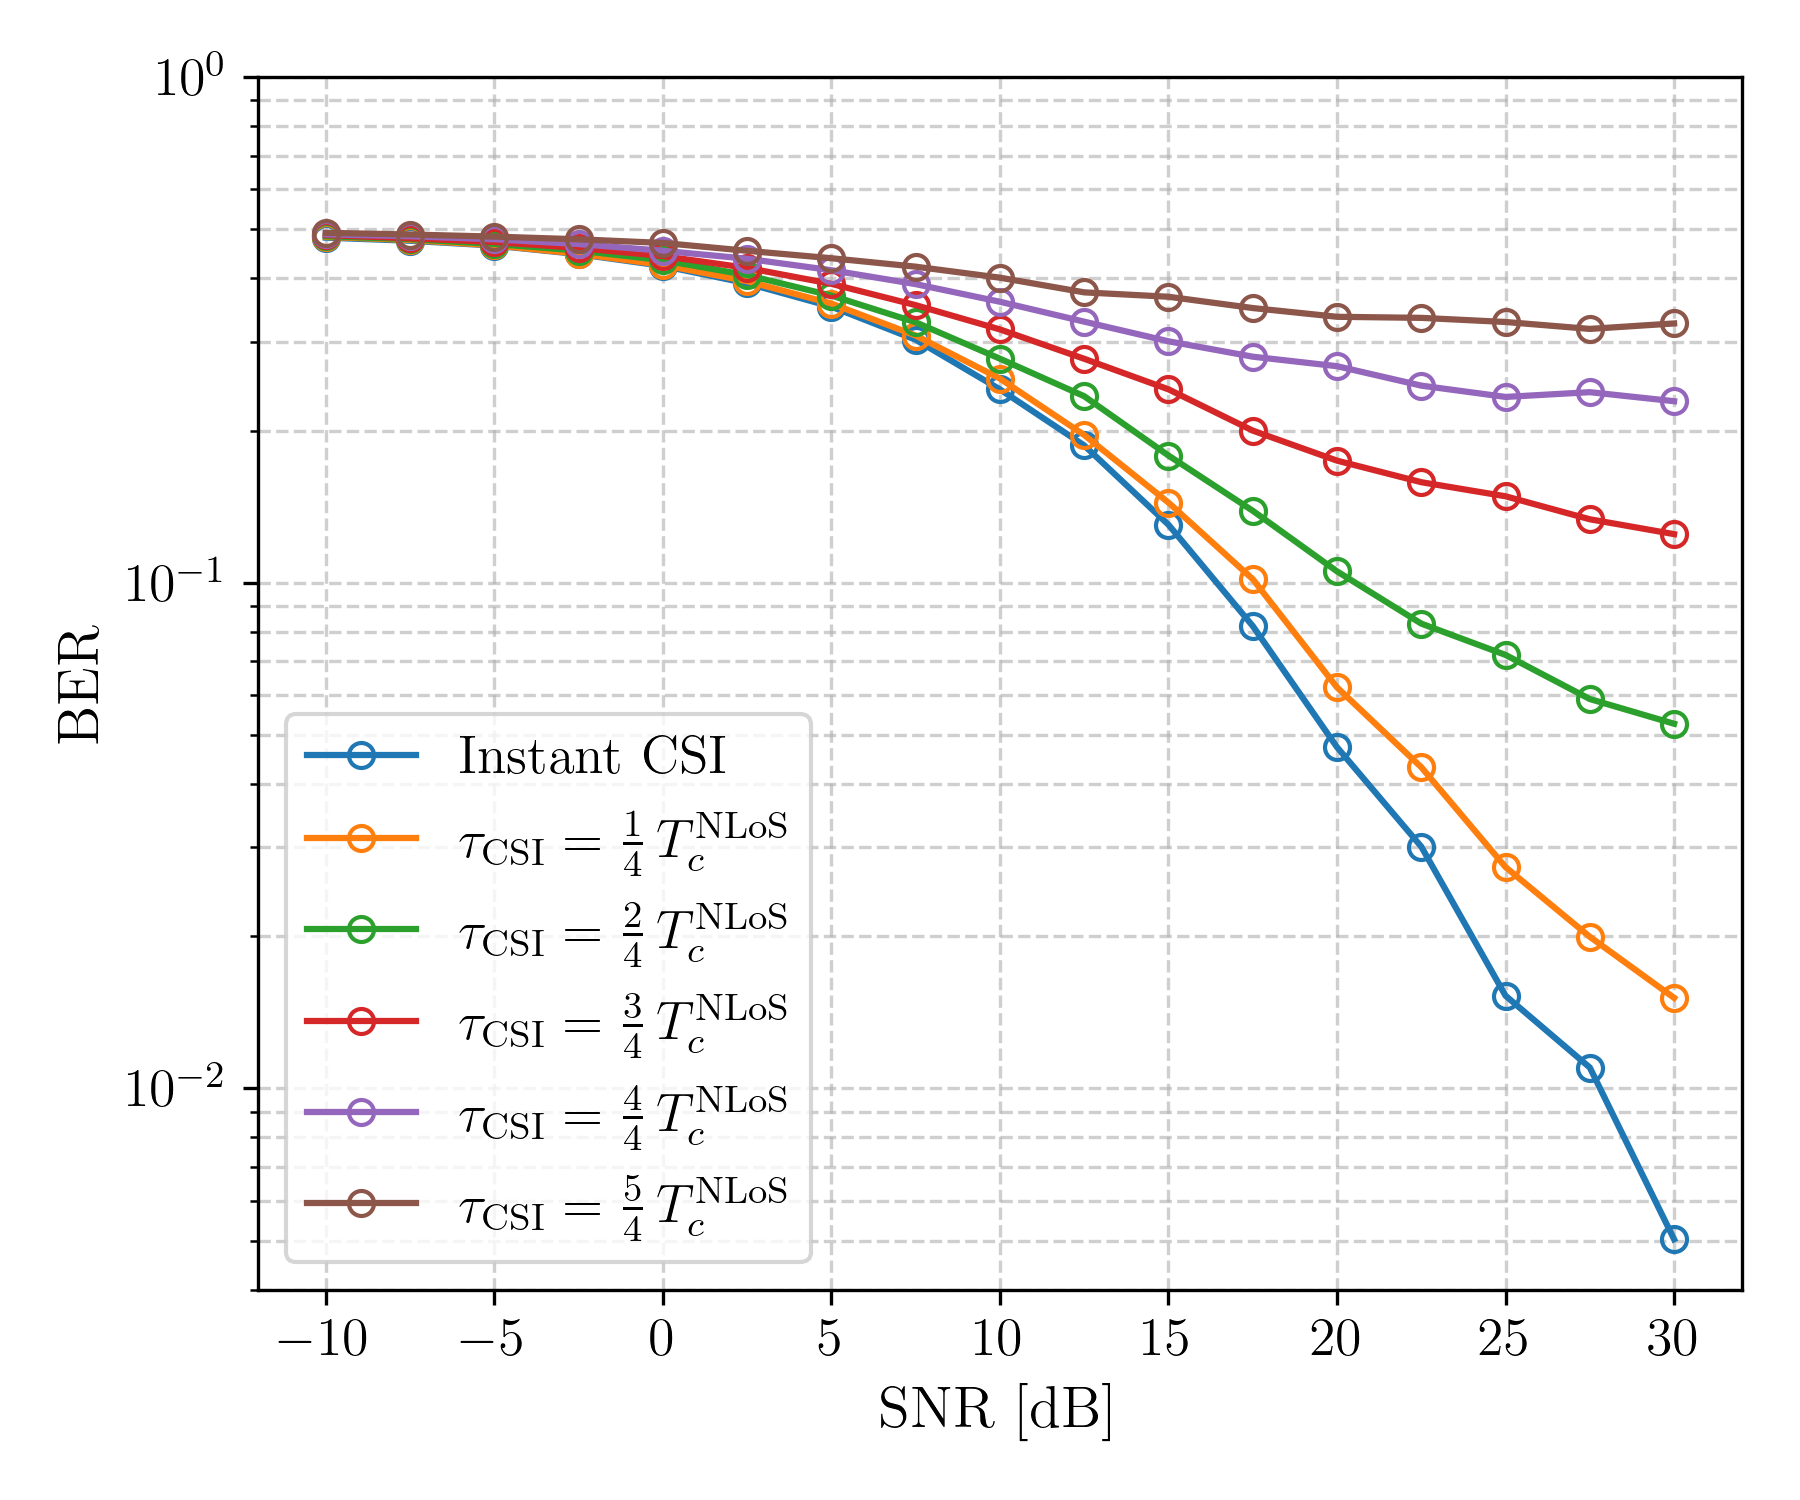
\includegraphics[width=\textwidth]{figures/mobile_satellite_systems/06_precoding_under_outdated_csi/satellite_channel/impact_outdated_csi/ber_zf.png}
        \caption{Outdated \acs{CSI}}
        \label{fig:satellite_channel_impact_outdated_csi_ber_zf}
    \end{subfigure}
    \hfill
    \begin{subfigure}{0.495\textwidth}
        \centering
        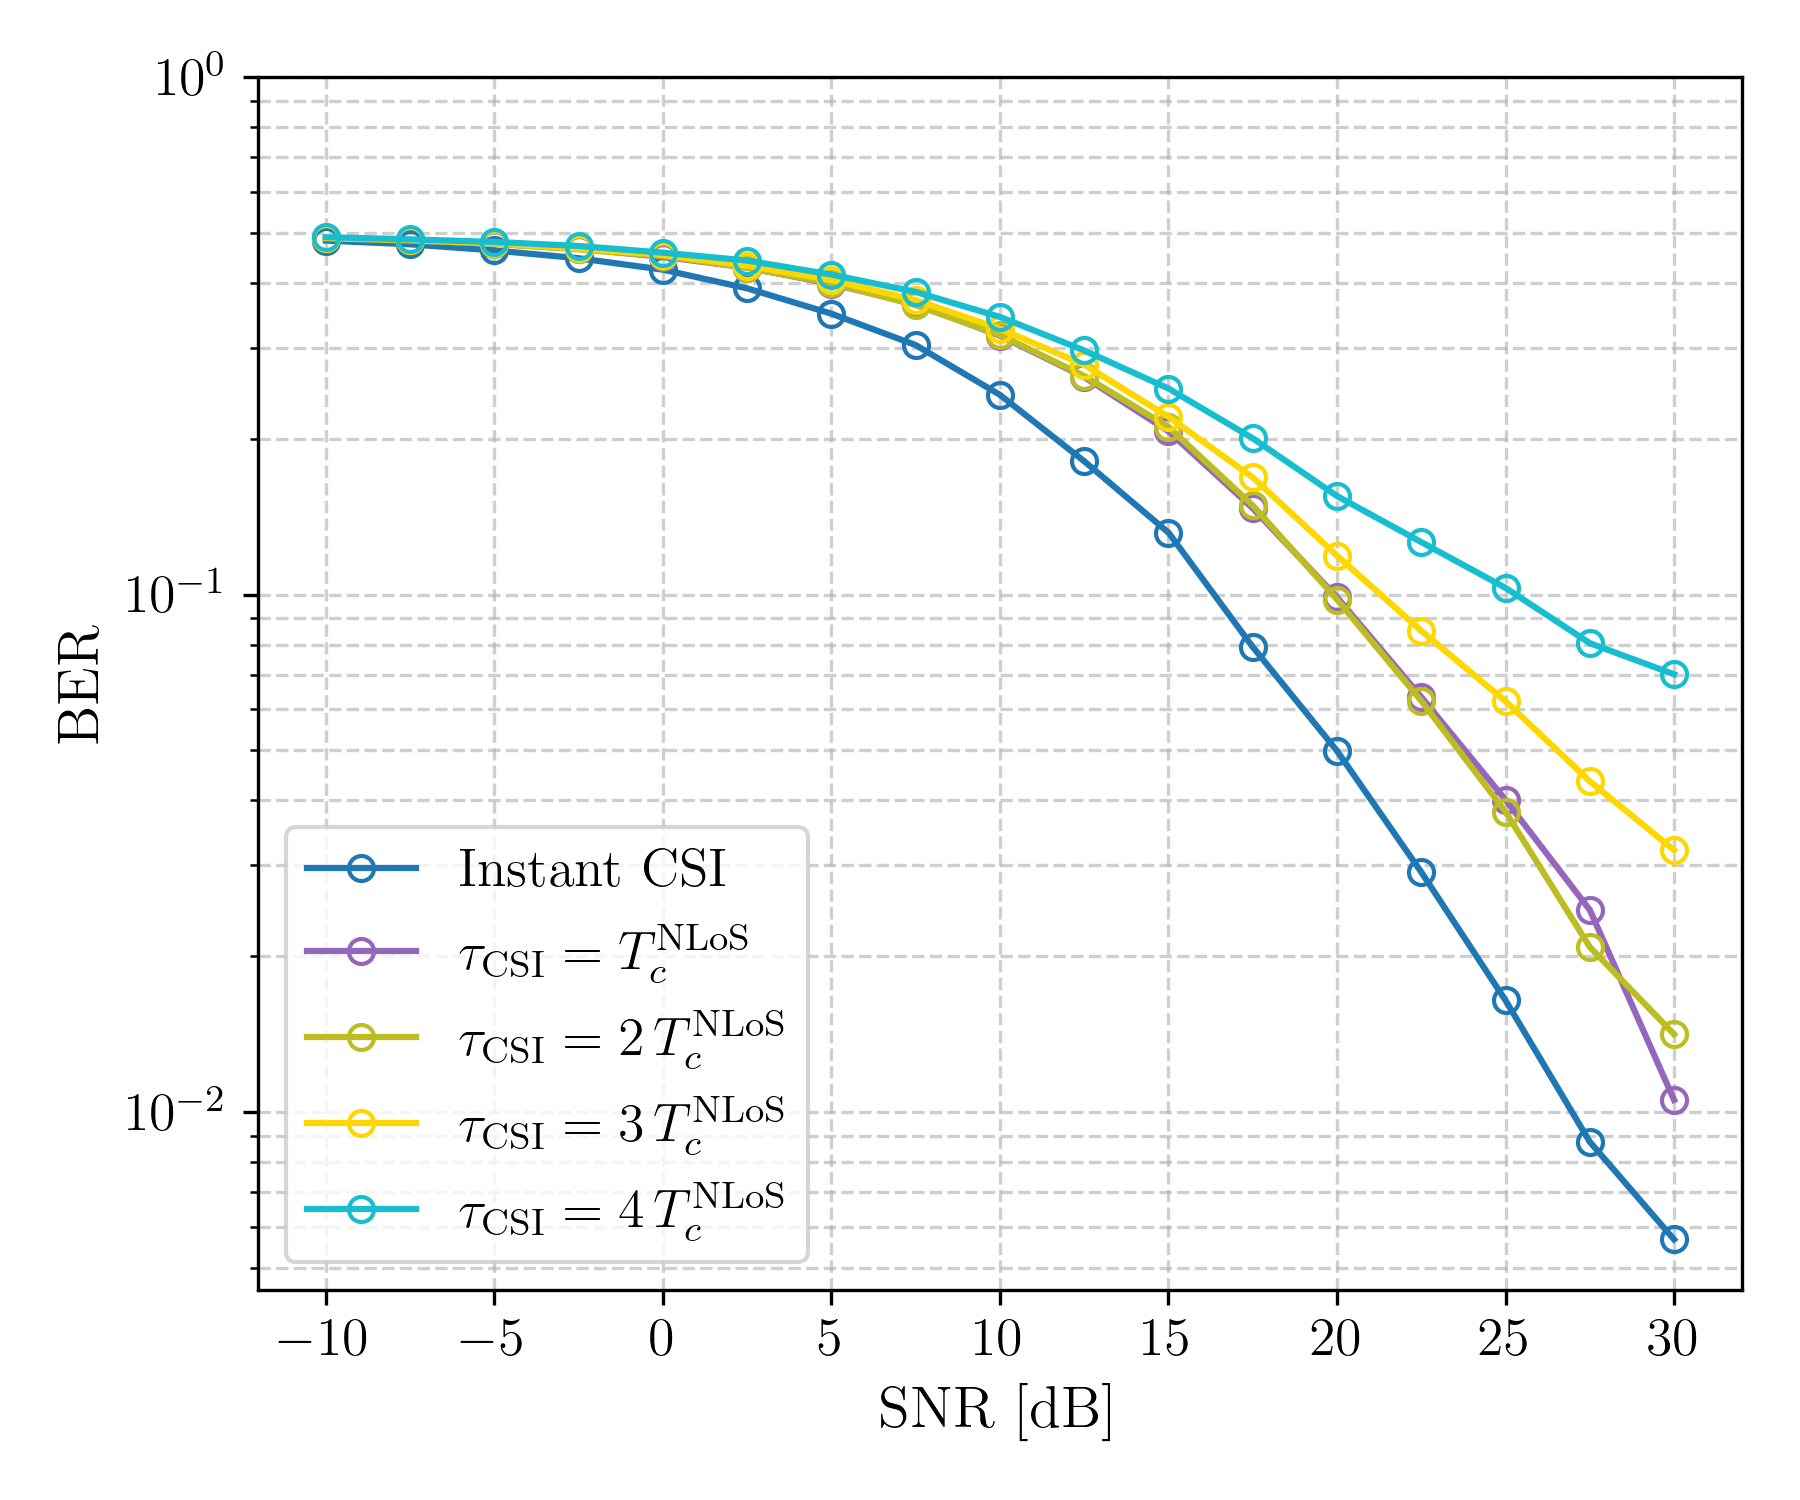
\includegraphics[width=\textwidth]{figures/mobile_satellite_systems/06_precoding_under_outdated_csi/satellite_channel/impact_compensation/ber_zf.png}
        \caption{Predicted \acs{CSI}}
        \label{fig:satellite_channel_impact_compensation_ber_zf}
    \end{subfigure}
    \caption[Impact of Outdated and Predicted \acs{CSI} on the \acs{BER} (\acs{ZF} precoding)]{
        A comparison of the total \acs*{BER} in a $8 \times \{1,1,1,1\}$ system using a \ac{ZF} precoder.
        The \acs*{BS} transmits a single $16$--\acs*{QAM} data stream to each \acs*{UT}.
        The different colored curves correspond to different \acs*{CSI} feedback delays.
    }
    \label{fig:satellite_channel_performance}
\end{figure}

\section{Conclusion}
\label{section:conclusion}
% ====================
%     Conclusion
% ====================

This chapter addressed a major limitation of linear precoding in mobile satellite systems: the \ac{CSI} used at the \ac{GW} is inevitably outdated at transmission time.
After restating the problem in terms of the normalized delay $\tau_{\mathrm{CSI}}/T_c$, we quantified the resulting mismatch, proposed a compensation strategy based on channel prediction at the \acp{UT}, and evaluated its robustness under a more realistic ray-based satellite channel model.

The analysis of Section~\ref{section:outdated_csi_impact} showed that all considered precoders are highly sensitive to \ac{CSI} aging.
Even moderate delay values cause a substantial loss at medium and high \ac{SNR}, and once $\tau_{\mathrm{CSI}}$ approaches the coherence time of the \ac{NLoS} component, the system becomes strongly interference-limited.

To mitigate this effect, Section~\ref{section:outdated_csi_compensation} introduced an element-wise \ac{AR} predictor at the \acp{UT}, with unchanged precoding processing at the \ac{GW}.
After tuning the pilot rate and context window, the proposed strategy was shown to recover most of the performance loss for delays up to about one coherence time, and to remain beneficial beyond that range.
Hence, channel prediction offers a practical and low-complexity way to extend the operating region of linear precoding under delayed \ac{CSI} feedback.

Section~\ref{section:realistic_channel_evaluation} then replaced the simplified Rician model by a ray-based model including spatial correlation and residual \ac{LoS} Doppler.
The same compensation mechanism still provided clear performance gains.
The additional limitation caused by the user channel being rank-deficient was avoided by restricting the evaluation to single-antenna \acp{UT}.
\bigskip

Finally, let us map the normalized-delay results to representative \ac{MSS} operating points to provide a more practical insight.
The total \ac{CSI} feedback delay is modelled as four times the one-way propagation delay between the \ac{UT} and the satellite. This factor of four accounts for the downlink pilot transmission to the \acp{UT}, the transmission of the estimated or predicted channel over the return link from the \ac{UT} to the \ac{GW} through the satellite, and finally the transmission of the precoder matrix over the forward feeder link back to the satellite.
\ac{MSS} typically operate in the $L$-band~\cite{1_signal_processing_for_satellites}, with carrier frequencies between $1$ and $2~\mathrm{GHz}$, and corresponding wavelengths ranging from $15$ to $30~\mathrm{cm}$.
Table~\ref{tab:coherence_times} summarizes the maximum Doppler frequency and the \ac{NLoS} coherence time for different \ac{UT} velocities.
\begin{table}[!htb]
    \centering
    \renewcommand{\arraystretch}{1.25}
    \setlength{\tabcolsep}{10pt}

    \begin{tabular}{>{\centering\arraybackslash}m{3.2cm}|>{\centering\arraybackslash}m{2.8cm}>{\centering\arraybackslash}m{2.8cm}}
        \hline
        \textbf{UT velocity} & $f_D$ & $T_c^{\mathrm{NLoS}}$ \\
        \hline
        $5~\mathrm{km/h}$  & $6.95~\mathrm{Hz}$  & $34.84~\mathrm{ms}$ \\
        $15~\mathrm{km/h}$ & $20.85~\mathrm{Hz}$ & $11.61~\mathrm{ms}$ \\
        $20~\mathrm{km/h}$ & $27.80~\mathrm{Hz}$ & $8.71~\mathrm{ms}$  \\
        $30~\mathrm{km/h}$ & $41.70~\mathrm{Hz}$ & $5.81~\mathrm{ms}$  \\
        $40~\mathrm{km/h}$ & $55.59~\mathrm{Hz}$ & $4.36~\mathrm{ms}$  \\
        \hline
    \end{tabular}

    \caption[\acs{NLoS} coherence time at $f_c = 1.5~\mathrm{GHz}$ (L-band) for various \ac{UT} velocities]{
        The maximum Doppler frequency $f_D$ and \ac{NLoS} coherence time $T_c^{\mathrm{NLoS}}$ as a function of \ac{UT} velocity, for a carrier frequency in the L-band ($f_c = 1.5~\mathrm{GHz}$).
    }
    \label{tab:coherence_times}
\end{table}

For a \ac{LEO} satellite at an altitude of $550~\mathrm{km}$, the one-way propagation delay is $\tau_{\mathrm{prop}} = 1.84~\mathrm{ms}$, which results in a total \ac{CSI} feedback delay of $\tau_{\mathrm{CSI}} = 7.34~\mathrm{ms}$.
Comparing this value against Table~\ref{tab:coherence_times}, the condition $\tau_{\mathrm{CSI}} \leq T_c$ is satisfied for all \ac{UT} moving slower than approximately $20~\mathrm{km/h}$.
In this regime, the \ac{AR}-based compensation operates at its most effective and the achievable rate is restored to near-perfect-\ac{CSI} performance.
For higher velocities, such as $30~\mathrm{km/h}$ or $40~\mathrm{km/h}$, the feedback delay exceeds the coherence time and perfect restoration is no longer possible.
However, the compensation still provides a substantial gain: whereas uncompensated outdated \ac{CSI} would render the system essentially unusable at these speeds, the predicted \ac{CSI} preserves a meaningful link quality.
The \ac{AR}-based strategy is therefore well-suited to \ac{LEO} satellite scenarios across a wide range of \ac{UT} velocities, under the assumption of a Rician fading channel as in~\ref{eq:rician_channel_model}.

For a \ac{GEO} satellite at an altitude of $35\,786~\mathrm{km}$, the one-way propagation delay is $\tau_{\mathrm{prop}} = 119.4~\mathrm{ms}$, yielding $\tau_{\mathrm{CSI}} = 477.5~\mathrm{ms}$.
Even for the slowest \ac{UT} velocity considered ($5~\mathrm{km/h}$, $T_c = 34.84~\mathrm{ms}$), this corresponds to $\tau_{\mathrm{CSI}} / T_c \approx 13.7$, far beyond the range where temporal prediction is effective.
The \ac{AR}-based compensation strategy is therefore not applicable to \ac{GEO} links.
In this regime, the mismatch between the available and the actual channel is too large to be bridged by the predictor.
More robust precoding formulations that explicitly account for severe \ac{CSI} uncertainty are required.
